\documentclass[12pt]{article}
\usepackage{amsmath}
\usepackage{amssymb}
\usepackage{amsthm}
\usepackage[left=2cm, right=2cm, top=2cm]{geometry}
\usepackage{enumitem}
\usepackage{graphicx}
\usepackage{color}   %May be necessary if you want to color links
\usepackage{hyperref}
\hypersetup{
    colorlinks=true, %set true if you want colored links
    linktoc=all,     %set to all if you want both sections and subsections linked
    linkcolor=blue,  %choose some color if you want links to stand out
}
\usepackage{bbm}
\usepackage{soul}
\usepackage{tcolorbox}
\usepackage{tikz}
\tcbuselibrary{theorems}
\tcbuselibrary{breakable}

\newtcbtheorem[number within=section]{mythm}{Theorem}%
{colback=green!5,colframe=green!35!black,fonttitle=\bfseries,unbreakable}{th}
\newtcbtheorem[use counter from=mythm]{mydef}{Definition}%
{colback=blue!5,colframe=blue!35!black,fonttitle=\bfseries,unbreakable}{de}
\newtcbtheorem[use counter from=mythm]{myrem}{Remark}%
{colback=white!5,colframe=white!35!black,fonttitle=\bfseries,unbreakable}{re}
\newtcbtheorem[use counter from=mythm]{myex}{Example}%
{colback=orange!5,colframe=orange!35!black,fonttitle=\bfseries,unbreakable}{ex}
\newtcbtheorem[use counter from=mythm]{myprop}{Proposition}%
{colback=green!5,colframe=green!35!black,fonttitle=\bfseries,unbreakable}{pr}
\newtcbtheorem[use counter from=mythm]{mylem}{Lemma}%
{colback=green!5,colframe=green!35!black,fonttitle=\bfseries,unbreakable}{le}
\newtcbtheorem[use counter from=mythm]{mycor}{Corollary}%
{colback=green!5,colframe=green!35!black,fonttitle=\bfseries,unbreakable}{co}

\newcommand{\R}{\mathbb{R}}
\newcommand{\N}{\mathbb{N}}
\newcommand{\Z}{\mathbb{Z}}
\newcommand{\Q}{\mathbb{Q}}
\renewcommand{\C}{\mathbb{C}}
\newcommand{\inv}{^{-1}}
\renewcommand{\Im}{\text{Im }}
\newcommand{\Stab}{\text{Stab}}

\setcounter{tocdepth}{3}
\setlength\parindent{0pt}
\hyphenpenalty 10000

\title{PMATH 336 Course Notes - Spring 2019}
\author{Max Zhu}

\begin{document}
	\maketitle
	\tableofcontents\newpage
	
	\section{Groups}
	\subsection{Definition and simple examples}
	Groups are used for describing symmetries of objects, and for finding solutions to equations. Before formally defining what a group is, we will start with some examples and note their properties.
	\begin{myex}{Integers with addition}{}
		$(\Z, +)$, the integers with usual addition, is a group. We notice the following properties.
		\begin{itemize}
			\item For all $a, b\in\Z$ we have $a+b\in\Z$. \textbf{(closure)}
			\item There is an identity $0\in\Z$ such that for all $a\in\Z$, we have $a+0=0+a=a$. \textbf{(identity)}
			\item Every integer $a\in\Z$ has an inverse $a\inv\in\Z$ such that $a+a\inv=a\inv+a=0$. Here, $a\inv=-a$. \textbf{(inverses)}
			\item Let $a, b, c\in\Z$. Then, $(a+b)+c=a+(b+c)$. \textbf{(associativity)}
		\end{itemize}
	\end{myex}
	
	\begin{myex}{Rationals with addition}{}
		$(\Q, +)$, rational numbers with usual addition, is a group. Similarly to the integers,
		\begin{itemize}
			\item For all $a, b\in\Q$ we have $a+b\in\Q$. \textbf{(closure)}
			\item There is an identity $0\in\Q$ such that for all $a\in\Q$, we have $a+0=0+a=a$. \textbf{(identity)}
			\item Every integer $a\in\Q$ has an inverse $a\inv\in\Q$ such that $a+a\inv=a\inv+a=0$. Here, $a\inv=-a$. \textbf{(inverses)}
			\item Let $a, b, c\in\Q$. Then, $(a+b)+c=a+(b+c)$. \textbf{(associativity)}
		\end{itemize}
	\end{myex}
	\begin{myex}{Real and complex numbers with addition}{}
		$(\R, +)$ and $(\C, +)$ are also groups, and these properties can be easily verified.
	\end{myex}
	
	\begin{myex}{}{}
		$(\{1, 1, i, -i\}, \cdot)$ is a group. We can create a table to show the result of the operation on any two elements of the set:
		\begin{align*}
			\begin{array}{c | cccc}
			\cdot & 1  & -1 & i  & -i \\
			\hline
			1     & 1  & -1 & i  & -i \\
			-1    & -1 & 1  & -i & i  \\
			i     & i  & -i & -1 & 1  \\
			-i    & -i & i  & 1  & -1
			\end{array}
		\end{align*}
		This kind of table is called a \underline{Cayley table}.
		\begin{itemize}
			\item Note that each row and column contains each element exactly once.
			\item From the Cayley table, the set is closed under $\cdot$.
			\item The identity is 1.
			\item Each element has an inverse in the set:\begin{align*}
				(1)\inv&=1\\
				(-1)\inv&=-1\\
				(i)\inv&=-i\\
				(-i)\inv&=i
			\end{align*}
		\end{itemize}
	\end{myex}
	
	\begin{mydef}{Group}{}
		Let $G$ be a set, and $\star:G\times G\to G$ be a binary operation on $G$. We say $(G, \star)$ is a \underline{group} if it satisfies the following conditions:
		\begin{enumerate}[label=(\roman*)]
			\item \underline{Associativity:} Let $a, b\in G$. Then, $(a\star b)\star c)=a\star(b\star c)$.
			\item \underline{Identity:} There exists $e\in G$ such that for all $a\in G$, we have $a\star e=e\star a=a$.
			\item \underline{Inverses:} For all $a\in G$, there exists $a\in\in G$ such that $a\star a\inv=a\inv\star a=e$.
		\end{enumerate}
	\end{mydef}
	
	\begin{myrem}{}{}
		\begin{itemize}
			\item When proving a set $G$ with an operation $\star$ is a group, we must also show $G$ is closed under $\star$.
			\item We often refer to a group $(G, \star)$ as simply $G$.
			\item We often write $ab$ instead of $a\star b$ for some operation $\star$.
			\item We usually denote the identity element of a group with $e$.
		\end{itemize}			
	\end{myrem}
	
	\begin{myprop}{Nonzero rationals with multiplication is a group}{}
		$(\Q\backslash\{0\}, \cdot)$, nonzero rationals with usual multiplication, is a group. 
		\begin{proof}
			We use the notation $\Q^*:=\Q\backslash\{0\}$.
			
			Let $a, b, c, d, e, f\in\Z$ so $\frac{a}{b}, \frac{c}{d}, \frac{e}{f}\in\Q^*$. Then,
			\begin{enumerate}[label=(\roman*)]
				\item $\frac{a}{b}\cdot\frac{c}{d}=\frac{ac}{bd}\in\Q^*$ \textbf{(closure)}
				\item $\frac{a}{b}\cdot(\frac{c}{d}\cdot\frac{e}{f})=(\frac{a}{b}\cdot\frac{c}{d})\cdot\frac{e}{f}$ \textbf{(associativity)}
				\item $\frac{1}{1}\cdot\frac{a}{b}=\frac{a}{b}\cdot\frac{1}{1}=\frac{a}{b}$ \textbf{(identity)}
				\item $\frac{a}{b}\cdot\frac{b}{a}=\frac{b}{a}\cdot\frac{a}{b}=\frac{1}{1}$, and $\frac{b}{a}\in\Q^*$ \textbf{(inverses)}
			\end{enumerate}
			So, $(\Q^*, \cdot)$ has all required properties of a group.
		\end{proof}
	\end{myprop}
	
	\begin{myex}{Integers modulo n with addition}{}
		$(\Z_n, +)$, integers modulo n with addition is a group.
		
		Here, $\Z_n=\{[0], \dots, [n-1]\}$ where $[a]=\{b\in\Z:b\text{ has remainder $a$ when dividing by n}\}$, and $[a]+[b]=[a+b]$. To save space, we may write $a$ instead of $[a]$. Let us use $\Z_5$ as an example.\\
		
		$\Z_5=\{0, 1, 2, 3, 4\}$. Here is the Cayley table for $\Z_5$:
		\begin{align*}
			\begin{array}{c | ccccc}
			+ & 0 & 1 & 2 & 3 & 4 \\
			\hline
			0 & 0 & 1 & 2 & 3 & 4 \\
			1 & 1 & 2 & 3 & 4 & 0 \\
			2 & 2 & 3 & 4 & 0 & 1 \\
			3 & 3 & 4 & 0 & 1 & 2 \\
			4 & 4 & 0 & 1 & 2 & 3
			\end{array}
		\end{align*}
		We can quickly verify the 4 properties. Let $[a], [b], [c]\in\Z_5$. Then,
		\begin{enumerate}[label=(\roman*)]
			\item Closure: obvious from the Cayley table.
			\item Associativity: $[a]+([b]+[c])=[a]+[b+c]=[a+b+c]=[a+b]+c=([a]+[b])+c$
			\item Identity: $[0]+[a]=[0+a]=[a]=[a+0]=[a]+[0]$
			\item Inverses: $[a]\inv=[-a]=[n-a]$
		\end{enumerate}
	\end{myex}
	
	\begin{myex}{``Integers modulo n" with multiplication}{}
		$(\Z_n^*, \cdot)$, where $\Z_n^*:=\{[a]\in\Z_n:\gcd(a, n)=1\}$ and $[a]\cdot[b]=[ab]$, is a group. Let us use $\Z_6^*$ as an example.\\
		
		$\Z_6^*=\{1, 5\}$. Note, $4\notin\Z_6^*$ since $2|4$ and $2|6$, so $\gcd(4, 6)=2\neq1$. Here is the Cayley table for $\Z_6^*$:
		\begin{align*}
			\begin{array}{c | cc}
			\cdot & 1 & 5 \\
			\hline
			1     & 1 & 5 \\
			5     & 5 & 1
			\end{array}
		\end{align*}
		Here, the identity is $1$ and the inverses are $(5)\inv=5$ and $(1)\inv=1$.
	\end{myex}
	
	\begin{myex}{General linear group in $\R$}{}
		We define the group $GL_n(\R)$ to be the set $\{A\in M_n(\R):\det(A)\neq0\}$ with usual matrix multiplication. We can easily verify the properties. Let $A, B\in GL_n(\R)$. Then,
		\begin{enumerate}[label=(\roman*)]
			\item Closure: $\det(AB)=\det(A)\det(B)\neq0$ so $AB\in GL_n(\R)$.
			\item Associativity: matrix multiplication is known to be associative.
			\item Identity: $\det(I)=1\neq0$ where $I=\begin{bmatrix}1&~&0\\~&\ddots\\0&~&1\end{bmatrix}$ is the identity matrix.
			\item Inverses: usual matrix inverses, since $\det(A\inv)=\frac{1}{\det(A)}\neq0$ so $A\inv\in GL_n(\R)$.
		\end{enumerate}
	\end{myex}
	
	\begin{mydef}{Abelian groups}{}
		A group $(G, \star)$ is \underline{abelian} if for all $a, b\in G$ we have $a\star b=b\star a$. Otherwise, the group is \underline{non-abelian}.	
	\end{mydef}
	
	\begin{myex}{Some abelian groups}{}
		$(\Z, +), (\Q^*, \cdot), (\Z_n, +), (\Z_n^*)$ are all abelian.
	\end{myex}
	
	\begin{myex}{Dihedral groups}{}
		\underline{Dihedral groups}	$(D_n, \cdot)$ are a family of groups of symmetries of a regular n-gon. The operations can be thought of as operations that change places of the vertices but not the overall shape of the polygon. Let us use $D_4$ as an example.\\
		
		$D_4$ is the group of symmetries of a square. Elements of $D_4$ include:
		\begin{itemize}
			\item $e$, rotation by 0\textdegree.
			\item $R$, rotation by 90\textdegree counter-clockwise.
			\item $R^2$, rotation by 180\textdegree counter-clockwise.
			\item $R^3$, rotation by 270\textdegree counter-clockwise.
		\end{itemize}
		We also have flips:
		\begin{itemize}
			\item $H$, flip through horizontal axis.
			\item $V$, flip through vertical axis.
			\item $D$, flip through top-left bottom-right diagonal axis.
			\item $D'$, flip through top-right bottom-left diagonal axis.
		\end{itemize}
		The elements are functions from a set of vertices to itself which preserves distance and adjacent-ness. The operator is composition of functions. For example, $HR$ is application of $R$ then $H$.
		
		\includegraphics[scale=0.3]{Fig1.png}
		
		From this MS Paint illustration of some operations in $D_4$, it is clear that $D_4$ is non-abelian.
	\end{myex}
	
	\begin{mydef}{Order of a group}{}
		Let $(G, \star)$ be a group. The \underline{order} of $G$ is the number of elements in $G$, which is denoted $|G|$. If $G$ is infinite, we say $|G|=\infty$.	
	\end{mydef}
	
	\begin{myex}{Orders of some groups}{}
		\begin{align*}
			|Z_n|&=n\\
			|Z_n^*|&=\phi(n)\text{ (Euler's totient function)}\\
			|(\Z, +)|&=\infty\\
			|D_n|&=2n
		\end{align*}			
	\end{myex}
	
	\subsection{Properties of groups}
	\begin{myprop}{Uniqueness of identity}{}
		In a group $G$, there is only one identity element.
		\begin{proof}
			Assume there are 2 identities $e, f\in G$. Since $e$ is an identity,
			\begin{align*}
				ef=fe&=f
			\end{align*}
			And since $f$ is an identity,
			\begin{align*}
				fe=ef&=e
			\end{align*}
			Therefore $e=f$.
		\end{proof}			
	\end{myprop}
	
	\begin{myprop}{Uniqueness of inverses}{}
		Let $G$ be a group. If $b, c$ are both inverses of $a$ then $b=c$.
		\begin{proof}
			Suppose $e=ab=ac$. Then,\begin{align*}
				ab&=ac\\
				b(ab)&=b(ac)\\
				(ba)b&=(ba)c\text{ [associativity]}\\
				eb&=ec\text{ [by hypothesis]}\\
				b&=c\text{ [identity]}
			\end{align*}
			as required.
		\end{proof}	
	\end{myprop}
	
	\begin{myprop}{Cancellation}{}
		If $G$ is a group, for all $a, b, c\in G$ we have:
		\begin{align*}
			ab=ac&\Longrightarrow b=c\text{ [Left cancellation]}\\
			ba=ca&\Longrightarrow b=c\text{ [Right cancellation]}
		\end{align*}
		\begin{proof}
			Let $a, b, c\in G$ such that $ab=ac$. Then,
			\begin{align*}
				ab&=ac\\
				a\inv(ab)&=a\inv(ac)\\
				(a\inv a)b&=(a\inv a)c\text{ [associativity]}\\
				eb&=ec\text{ [inverses]}\\
				b&=c\text{ [identity]}
			\end{align*}
			As required. Right cancellation has similar proof.
		\end{proof}
	\end{myprop}
	
	\begin{myrem}{}{}
		Cancellation should be on the same side. For example in $D_4$, $RH=D'=VR$ but $H\neq V$.	
	\end{myrem}
	
	\begin{myprop}{Socks-shoes}{}
		Let $G$ be a group with $a, b\in G$. Then, $(ab)\inv=b\inv a\inv$.
		\begin{proof}
			\begin{align*}
				(ab)(b\inv a\inv)&=a(bb\inv)a\inv\\
				&=a(ea\inv)\\
				&=aa\inv\\
				&=e
			\end{align*}
			so $(ab)\inv=b\inv a\inv$ as required.
		\end{proof}			
	\end{myprop}
	
	\begin{mydef}{Exponentiation}{}
		Let $(G, \star)$ be a group, with $a\in G$, $n\in\Z$. Then,
		\begin{align*}
			a^n:=\begin{cases}
				\underbrace{a\star\dots\star a}_{\text{n times}},&n>0\\
				e,&n=0\\
				\underbrace{a\inv\star\dots\star a\inv}_{\text{n times}},&n<0
			\end{cases}
		\end{align*}
		
		Note: some exponential properties work. For example,
		\begin{align*}
			a^na^m&=a^{n+m}\\
			(a\inv)^n&=a^{-n}
		\end{align*}
		However, in general $(ab)^n\neq a^nb^n$ for $a. b\in G$ unless $G$ is abelian.
	\end{mydef}
	
	\begin{mydef}{Order of an element}{}
		Let $G$ be a group with $a\in G$. The \underline{order} of $a$ is the smallest positive integer such that $a^k=e$. We denote this by $|a|=k$. If $a^k\neq e$ for all $k\in\Z$, we say $|a|=\infty$.
	\end{mydef}
	
	\begin{myex}{Some orders of group elements}{}
		\begin{itemize}
			\item In all groups, $|e|=1$\\
			\item In $D_4$, $|V|=2$\\
			\item In $\Z_{15}^*$, $|2|=4$\\
			\item In $\Z$, all nonzero elements have order $\infty$\\
			\item In $\Q^*$, $|1|=1$ and $|-1|=2$
		\end{itemize}			
	\end{myex}
	
	\begin{mydef}{Direct products}{}
		Let $(G, \star), (H, \cdot)$ be groups. Then, the set $G\times H=\{(g, h):g\in G, h\in H\}$ with operation $(g_1, h_1)\Delta(g_2, h_2):=(g_1\star g_2, h_1\cdot h_2)$ is a group. $(G\times H, \Delta)$ is called the \underline{direct product} of $G$ and $H$.
	\end{mydef}
	
	\subsection{Subgroups}
	\begin{mydef}{Subgroup}{}
		Let $(G, \star)$ be a group, and $H\subseteq G$. Then $H$ is a \underline{subgroup} of $G$ if $(H, \star)$ is a group.\\
		
		If $H$ is a subgroup of $G$, we say $H\leq G$ and if $H\subsetneq G$, we say $H<G$.\\
		
		If 	$(H, \star)$ is not a group, we say $H\nleq G$.
	\end{mydef}
	
	\begin{myex}{Some easy subgroups}{}
		For all groups $(G, \star)$, we know $\{e\}\leq G$ and $G\leq G$.
	\end{myex}
	
	\begin{myex}{Subgroups of $\Z$}{}
		Define $n\Z=\{nk:k\in\Z\}$ for $n\in\Z$. Then, $(n\Z, +)$ is a group, so $n\Z\leq\Z$.
	\end{myex}
	
	\begin{myprop}{One-step test}{}
		Let $G$ be a group, and $\emptyset\neq H\subseteq G$. If for all $a, b\in H$ we have $ab\inv\in H$, then $H\leq G$.
		\begin{proof}
			Let $a, b\in H$, since $H\neq\emptyset$.
			\begin{enumerate}[label=(\roman*)]
				\item Associativity: follows from $G$ being a group.
				\item Identity: By hypothesis $aa\inv\in H$, so $e\in H$.
				\item Inverses: We know $e\in H$, so by hypothesis $ea\inv\in H$ so $a\inv\in H$.
				\item Closure: By inverses $b\inv\in H$, so by hypothesis $a(b\inv)\inv\in H$ thus $ab\in H$.
			\end{enumerate}
			So $H$ satisfies all requirements of a group.
		\end{proof}
	\end{myprop}
	
	\begin{myprop}{Two-step test}{}
		Let $(G, \star)$ be a group, and $\emptyset\neq H\subseteq G$. If $a, b\in H\Longrightarrow ab\in H$ and $a\in H\Longrightarrow a\inv\in H$, then $H\leq G$.
		
		In other words, $H\leq G$ iff $H$ is closed under $\star$ and closed under inverses.
		\begin{proof}
			Let $a, b\in H$, since $H\neq\emptyset$.
			\begin{enumerate}[label=(\roman*)]
				\item Associativity: follows from $G$ being a group.
				\item Identity: by hypothesis, $a\inv\in H$. Therefore, $aa\inv=e\in H$.
				\item Inverses: by hypothesis.
				\item Closure: by hypothesis.
			\end{enumerate}
			So $H$ satisfies all requirements of a group.
		\end{proof}
	\end{myprop}
	
	\begin{myex}{Center of a group}{}
		The \underline{center} of a group $G$ is defined $$Z(G):=\{a\in G:ag=ga\text{ for all }g\in G\}$$
		and is a subgroup of $G$.
		\begin{proof}
			Let $g\in G$ and $a, b\in Z(G)$. We know $eg=ge$ for all $g\in G$, so $Z(G)\neq\emptyset$. Now,
			\begin{align*}
				(ab)g&=a(bg)\\
				&=a(gb)\\
				&=(ag)b\\
				&=(ga)b\\
				&=g(ab)
			\end{align*}
			So $ab\in Z(G)$. Also, since $a\in Z(G)$,
			\begin{align*}
				ax&=xa\\
				a\inv(ax)&=a\inv(xa)\\
				(a\inv a)x&=a\inv(xa)\\
				ex&=a\inv(xa)\\
				x&=a\inv(xa)\\
				xa\inv&=a\inv(xa)a\inv\\
				xa\inv&=(a\inv x)(aa\inv)\\
				xa\inv&=(a\inv x)e\\
				xa\inv&=a\inv x
			\end{align*}
			So $a\inv\in Z(G)$. By two-step test, $Z(G)\leq G$.
		\end{proof}
		
		Note: A group $G$ is abelian iff $Z(G)=G$.
	\end{myex}
	
	\begin{myex}{Centralizer of a group element}{}
		The \underline{centralizer} of an element of a group $g\in G$ is defined $$C(g):=\{a\in G:ag=ga\}$$
		and is a subgroup of $G$.
		\begin{proof}
			Let $g\in G$ and $a, b\in C(g)$. Then,
			\begin{align*}
				bg&=gb\\
				b\inv bg&=b\inv gb\\
				b\inv bgb\inv&=b\inv gbb\inv\\
				gb\inv&=b\inv g\\
				\therefore b\inv&\in C(g)
			\end{align*}
			so $C(g)$ is closed under inverses. Also,
			\begin{align*}
				(ab)g&=a(bg)\\
				&=a(gb)\\
				&=(ag)b\\
				&=(ga)b\\
				&=g(ab)\\
				\therefore ab&\in C(g)
			\end{align*}
			so $C(g)$ is closed under the group operation. By two-step test, $C(g)\leq G$ for all $g\in G$.
		\end{proof}
		
		Note: $Z(G)=\bigcap_{g\in G}C(g)$.
	\end{myex}
	
	\begin{myrem}{Aside}{}
		The definition of centralizer was not given here in the original notes but it is used later and makes most sense to be here.
	\end{myrem}
	
	\begin{mydef}{Generator of a group}{}
		Let $G$ be a group, with $a\in G$. Then, $\langle a\rangle:=\{a^n:n\in\Z\}$. This is the \underline{(sub)group generated by $a$} and $a$ is called the \underline{generator} of this group.
	\end{mydef}
	
	\begin{myrem}{}{}
		Not all subgroups are generated by a single element. For example, if $H=\{(0, 0), (0, 2), (2, 0), (2, 2)\}$ then $H\leq\Z_4\times\Z_4$ but $H$ is not generated by any of its elements.
	\end{myrem}
	
	\section{Lagrange's theorem}	
	\subsection{Cosets}
	\begin{mydef}{Coset}{}
		Let $G$ be a group and $H\leq G$.
		
		For any $a\in G$, $$aH:=\{ah:h\in H\}$$ is the \underline{left coset of $H$ containing $a$ in $G$} and $$Ha:=\{ha:h\in H\}$$ is the \underline{right coset of $H$ containing $a$ in $G$}. We denote the number of left cosets of $H$ in $G$ by $|G:H|$, and call it the \underline{index of $H$ in $G$}.
	\end{mydef}
	
	\begin{myex}{Cosets of $\Z_9$}{}
		Let $G=\Z_9$, $H=\{0, 3, 6\}=\langle 3\rangle$. Then,
		\begin{align*}
			0+H&=\{0, 3, 6\}=3+H=6+H\\
			1+H&=\{1, 4, 7\}=4+H=7+H\\
			2+H&=\{2, 5, 8\}=5+H=8+H\\
		\end{align*}
		We can make several observations.
		\begin{itemize}
			\item $aH$ may not be a group.
			\item $aH$ may be equal to $bH$ even if $a\neq b$.
			\item All cosets are the same size.
			\item No element is in two different cosets.
		\end{itemize}
		We will use some of these observations to prove Lagrange's theorem.
	\end{myex}
	
	\begin{mylem}{}{3.3}
		Let $G$ be a group and $H\leq G$. Every element of $G$ is in some left coset of $H$.
		\begin{proof}
			Let $a\in G$. Then, $a=ae$ and $e\in H$ so $a\in aH$.
		\end{proof}
	\end{mylem}
	
	\begin{mylem}{}{3.4}
		Let $G$ be a group and $H\leq G$. Let $a, b\in G$. Then, $aH=bH$ or $aH\cap bH=\emptyset$.
		\begin{proof}
			Assume $aH\cap bH\neq\emptyset$. We will show that $aH=bH$.
			
			By hypothesis there is $c\in aH\cap bH$, so $c=ah_1=bh_2$ for $h_1, h_2\in H$. Let $ah\in aH$ for some $h\in H$. Then,
			\begin{align*}
				ah&=aeh\\
				&=a(h_1h_1\inv)h\\
				&=(ah_1)(h_1\inv h)\\
				&=bh_2h_1\inv h
			\end{align*}
			So $ah\in bH$ since $h_2h_1\inv h\in H$. Thus $aH\subseteq bH$ and similarly $bH\subseteq aH$. Therefore, $aH=bH$.
		\end{proof}
	\end{mylem}
	
	\begin{mylem}{}{3.5}
		Let $G$ be a group and $H\leq G$. Any left coset of $H$ has the same number of elements as $H$.
		\begin{proof}
			Let $a\in G$. We will show $|aH|=|H|$.
			
			Let $f:H\to aH$ be defined $f(h):=ah$ for all $h\in H$. Then,
			\begin{itemize}
				\item $f$ is injective: Let $h_1, h_2\in H$. Then, $f(h_1)=f(h_2)\Longrightarrow ah_1=ah_2\Longrightarrow h_1=h_2$ by cancellation.
				\item $f$ is surjective: Let $ah\in aH$. Then, $f(h)=ah$.
			\end{itemize}
			So $f$ is a bijection between $H$ and $aH$, so $|aH|=|H|$.
		\end{proof}		
	\end{mylem}
	
	\subsection{Lagrange's theorem and its corollaries}	
	\begin{mythm}{Lagrange's theorem}{Lagrange}
		Let $G$ be a finite group, and $H\leq G$. Then, $|H|$ divides $|G|$.
		\begin{proof}
			By lemmas \ref{le:3.3} and \ref{le:3.4}, there exist $a_1, \dots, a_k\in G$ such that $G$ is a disjoint union of cosets: $G=a_1H\cup\dots\cup a_kH$. By lemma \ref{le:3.5},
			\begin{align*}
				|G|&=|a_1H|+\dots+|a_kH|\\
				&=|H|+\dots+|H|\\
				&=kH
			\end{align*}
			Therefore $|H|$ divides $|G|$.
		\end{proof}
	\end{mythm}
	
	\begin{mycor}{}{3.7}
		Let $G$ be a finite group. Then,
		\begin{enumerate}[label=(\roman*)]
			\item Let $H\leq G$. The index $|G:H|=\frac{|G|}{|H|}$.
			\item Let $a\in G$. Then, $|a|$ divides $|G|$.
			\item If $|G|$ is prime, then $G=\langle a\rangle$ for some $a\in G$.
			\item Let $a\in G$. Then, $a^{|G|}=e$.
			\item  \textbf{(Fermat's little theorem.)} Let $a\in\Z$, and $p$ be prime. then, $a^p\equiv a\mod p$.
		\end{enumerate}
		\begin{proof}~
			\begin{enumerate}[label=(\roman*)]
				\item Follows immediately from proof of Lagrange's theorem.
				\item We know $\langle a\rangle\leq G$. Since $|\langle a\rangle|=|a|$, the statement follows from Lagrange's theorem.
				\item Let $a\in G$ with $a\neq e$. This is possible since $|G|\geq2$. Then, $|a|$ divides $|G|$ by (ii). Since $a\neq e$ and $|G|$ is prime, $|a|=|G|$. So, since $|\langle a\rangle|=|G|$ and $\langle a\rangle\leq G$, we have $\langle a\rangle=G$.
				\item By (ii) we have $k|a|=|G|$ for some $k\in\Z$. So,
				\begin{align*}
					a^{|G|}&=a^{k|a|}\\
					&=(a^{|a|})^k\\
					&=e^k\\
					&=e
				\end{align*}
				\item Let $a\in\Z$. Then, if $p|a$ then $p|a^p\Longrightarrow a^p\equiv0\mod p$. If $p\nmid a$ then $\gcd(a, p)=1$. So, $a\equiv n\mod p$ for some $n\in\Z_p^*$. Now, $|\Z_p^*|=p-1$. By (iv) we have
				\begin{align*}
					n^{p-1}&\equiv1\mod p\\
					n^p&\equiv n\mod p\\
					a^p&\equiv a\mod p
				\end{align*}
			\end{enumerate}
		\end{proof}
	\end{mycor}
	
	\section{Cyclic groups}
	\begin{mydef}{Cyclic group}{}
		Let $G$ be a group. $G$ is \underline{cyclic} if there exists $a\in G$ such that $\langle a\rangle=G$. $a$ is then a \underline{generator} of $G$.
	\end{mydef}
	
	\begin{myex}{Some cyclic groups}{}
		\begin{itemize}
			\item $(\Z, +)$ is cyclic, since $\Z=\langle 1\rangle=\langle -1\rangle$.
			\item $\Z_6$ is cyclic, since $\Z_6=\langle 1\rangle=\langle 5\rangle$.
			\item $\Z_9^*$ is cyclic, since $\Z_9^*=\langle 2\rangle$.
		\end{itemize}
	\end{myex}
	
	\begin{myprop}{Cyclic groups are abelian}{}
		Let $G=\langle a\rangle$ be a cyclic group. Then $G$ is abelian.
		\begin{proof}
			Let $a^n, a^m\in G$ where $n, m\in\Z$. Then,
			\begin{align*}
				a^na^m&=a^{n+m}\\
				&=a^ma^n
			\end{align*}
		\end{proof}
	\end{myprop}
	
	\begin{myprop}{Subgroups of a cyclic group are cyclic}{4.4}
		Let $G=\langle a\rangle$ be a cyclic group, and $H\leq G$. Then $H$ is also cyclic.
		\begin{proof}
			If $G=\{e\}$, clearly $H=G$ so we're done. Thus assume $G\neq\{e\}$. So, $G=\langle a\rangle$ where $a\neq e$.\\
			
			Let $k$ be the smallest positive integer such that $a^k\in H$. Now, it is clear that $\langle a^k\rangle\subseteq H$ since $H$ is a group. Let $a^n\in H$ for some integer $n$. By division algorithm, $n=qk+r$ for $q, r\in\Z$ and $0\leq r<k$. So, $a^n=a^{kq+r}=(a^k)^q(a^r)$ which implies $(a^k)^{-q}a^n=a^r$. Since $a^k, a^n\in H$ we have $a^r\in H$. However, $r<k$ so $r=0$, since $k$ is the minimal positive integer such that $a^k\in H$. Therefore, $a^n=(a^k)^q$ so $H=\langle a^k\rangle$.
		\end{proof}
	\end{myprop}
	
	\begin{mythm}{Criterion for $a^i=a^j$}{4.5}
		Let $G$ be a group with $a\in G$.
		\begin{itemize}
			\item If $|a|=\infty$, then $a^i=a^j\Longleftrightarrow i=j$.
			\item If $|a|=n\in\N$, then
			\begin{enumerate}[label=(\roman*)]
				\item $\langle a\rangle=\{e, a, \dots, a^{n-1}\}$
				\item $a^i=a^j\Longleftrightarrow n|i-j$.
			\end{enumerate}
		\end{itemize}
		
		\begin{proof}~\\
			\begin{itemize}
				\item Suppose $a\in G$ such that $a^i=a^j$ and $|a|=\infty$. Then, $a^{i-j}=e$. However since $|a|=\infty$, we know $a^k\neq e$ for all $k\in\N$. So, $i-j=0$ and $i=j$. Trivially, $i=j\Longrightarrow a^i=a^j$.
				\item Suppose $a\in G$ and $|a|=n\in\N$.
				\begin{enumerate}[label=(\roman*)]
					\item We must prove that $\langle a\rangle\subseteq\{e, a, \dots, a^{n-1}\}$ (*) and $\{e, a, \dots, a^{n-1}\}\subseteq\langle a\rangle$ (**). (**) is trivial from definition of $\langle a\rangle$, so we will prove (*).\\
					
					Let $a^k\in\langle a\rangle$ for some $k\in\N$. If $k<n$ then clearly $a^k\in\{e, a, \dots, a^{n-1}\}$. Otherwise, there exists $q, r\in\Z$ such that $k=qn+r$ with $0\leq r<n$, by division algorithm. So, we have
					\begin{align*}
						a^k&=a^{nq+r}\\
						&=a^{nq}a^r\\
						&=(a^n)^qa^r\\
						&=e^qa^r\\
						&=a^r
					\end{align*}
					So since $0\leq r<n$, we have $a^k\in\{e, a, \dots, a^{n-1}\}$ so (i) holds.
					
					\item $(\Longrightarrow)$ We know $a^i=a^j\Longrightarrow a^{i-j}=e$. By division algorithm, $i-j=nq+r$ for $q, r\in\Z$ and $0\leq r<n$. So,
					\begin{align*}
						i-j&=nq+r\\
						a^{i-j}&=(a^n)^qa^r\\
						e&=a^r
					\end{align*}
					Since $|a|=n$, we know $n$ is the smallest positive integer such that $a^n=e$, and we know $r<n$, therefore $r=0$ and $i-j=nq$ for some $q\in\Z$.
					
					$(\Longleftarrow)$ If $i-j=nq$ for some $q\in\Z$, then $a^{i-j}=(a^n)^q=e\Longrightarrow a^i=a^j$.
				\end{enumerate}
			\end{itemize}
		\end{proof}
	\end{mythm}
	
	\begin{mycor}{}{}
		Suppose $|a|=n$. Then, $a^k=e$ iff $n|k$.
		\begin{proof}
			$a^k=e\Longleftrightarrow a^k=a^n\Longleftrightarrow n|k$ by theorem \ref{th:4.5}
		\end{proof}
	\end{mycor}
	
	\begin{myrem}{}{}
		Note that $a^k=e$ does not imply $k=|a|$. It does, however, imply $|a|$ divides $k$.
	\end{myrem}
	
	\begin{mythm}{}{4.8}
		Suppose $G$ is a cyclic group, with $G=\langle a\rangle$ and $|G|=|a|=n$. If $k\in\Z$, then
		\begin{enumerate}[label=(\roman*)]
			\item $\langle a^k\rangle=\langle a^{\gcd(n, k)}\rangle$
			\item $|\langle a^k\rangle|=\frac{n}{\gcd(n, k)}$
		\end{enumerate}
		\begin{proof}~\\
			\begin{enumerate}[label=(\roman*)]
				\item Let $d=\gcd(n, k)$. We want to prove $\langle a^k\rangle=\langle a^d\rangle$, and thus $\langle a^k\rangle\subseteq\langle a^d\rangle$ (*) and $\langle a^d\rangle\subseteq\langle a^k\rangle$ (**). By definition of $\gcd$, we know $k=rd$ for some $r\in\Z$. Then,
				\begin{align*}
					a^k&=a^{rd}\\
					&=(a^d)^r\in\langle a^d\rangle
				\end{align*}
				so (*) holds. To prove (**), it is enough to show $a^d\in\langle a^k\rangle$ since $d|k$. By B\'ezout's identity, there exist $s, t\in\Z$ such that $d=ns+kt$. So,
				\begin{align*}
					a^d&=a^{ns+kt}\\
					&=a^{ns}a^{kt}\\
					&=(a^n)^s(a^k)^t\\
					&=(a^k)^t
				\end{align*}
				Thus (**) holds and $\langle a^k\rangle=\langle a^{\gcd(n, k)}\rangle$.
				
				\item We want to prove $|a^d|=\frac{n}{d}$. Clearly $(a^d)^{\frac{n}{d}}=a^n=e$, so $|a^d|\leq\frac{n}{d}$. For contradiction suppose $|a^d|=\alpha<\frac{n}{d}$. Then,
				\begin{align*}
					(a^d)^\alpha&=e\\
					a^{d\alpha}&=e\\
					\alpha&<\frac{n}{d}\\
					d\alpha&<n
				\end{align*}
				But this contradicts $|a|=n$ so (ii) holds.
			\end{enumerate}
		\end{proof}
	\end{mythm}
	
	\begin{myex}{}{}
		Suppose $G=\langle a\rangle$ and $|a|=30$. What is $\langle a^{26}\rangle$?
		\begin{align*}
			\langle a^{26}\rangle&=\langle a^{\gcd(26, 30)}\rangle\\
			&=\langle a^2\rangle
		\end{align*}
		What about $\langle a^{23}\rangle$?
		\begin{align*}
			\langle a^{23}\rangle&=\langle a^{\gcd(23, 30)}\rangle\\
			&=\langle a\rangle
		\end{align*}
		Also, $|\langle a^{26}\rangle|=\frac{30}{2}=15$.
	\end{myex}
	
	\begin{mycor}{}{}
		$\Z_n$ is a cyclic group of order $n$, and $i\in\Z_n$ generates $\Z_n$ $\Longleftrightarrow$ $\gcd(i, n)=1$.
		\begin{proof}
			$(\Rightarrow)$ Suppose $\Z_n=\langle i\rangle$. Then, $|\langle i\rangle|=n$. By theorem \ref{th:4.8} this implies $\gcd(n, i)=1$.
			
			$(\Leftarrow)$ Suppose $\gcd(n, i)=1$. By theorem \ref{th:4.8} $|\langle i\rangle|=n$ so $\Z_n=\langle i\rangle$.
		\end{proof}
	\end{mycor}
	
	\begin{mythm}{Fundamental theorem of cyclic groups}{}
		Let $G$ be a finite cyclic group with $G=\langle a\rangle$ and $|G|=n$. Then,
		\begin{enumerate}
			\item Every subgroup of $G$ is cyclic.
			\item If $H\leq G$ then $|H|$ divides $|G|$.
			\item If $k$ is a divisor of $n$ then there is a unique subgroup $H\leq G$ such that $|H|=k$ and $H=\langle a^{\frac{n}{k}}\rangle$.
		\end{enumerate}
		\begin{proof}~\\
			\begin{enumerate}
				\item Proposition \ref{pr:4.4}
				\item Lagrange's theorem \ref{th:Lagrange}
				\item Suppose $k$ divides $n$. We need to prove there is a subgroup $H\leq G$ with $|H|=k$ (i) and that $H$ is the unique such subgroup (ii).
				\begin{enumerate}[label=(\roman*)]
					\item Consider $H=\langle a^{\frac{n}{k}}\rangle$. From theorem \ref{th:4.8}, $|H|=|\langle a^{\frac{n}{k}}\rangle|=\frac{n}{\gcd(n, \frac{n}{k})}$. Since $\frac{n}{k}|n$, we have $\gcd(n, \frac{n}{k})=\frac{n}{k}$. So, $|H|=\frac{n}{(n/k)}=k$.
					
					\item Suppose $P\leq G$ with $|P|=k$. From proposition \ref{pr:4.4}, $P=\langle a^m\rangle$ for some $m\in\N$. By theorem \ref{th:4.8}, $P=\langle a^{\gcd(n, m)}\rangle$. Since $|P|=k$ we have $\frac{n}{k}=\gcd(n, m)$ so $P=\langle a^{\frac{n}{k}}\rangle=H$.
				\end{enumerate}
			\end{enumerate}
		\end{proof}
	\end{mythm}
	
	\begin{myex}{Subgroups of $\Z_12$}{}
		We know $\Z_{12}=\langle 1\rangle$ and $|\Z_{12}|=12$. Here are the subgroups of $\Z_{12}$.
		
		\begin{tabular}{|l|l|}
		\hline
		Order & Subgroup \\ \hline
		1     & $\langle 1^{12}\rangle=\{0\}$\\ \hline
		2     & $\langle 1^{6}\rangle=\{0, 6\}$\\ \hline
		3     & $\langle 1^{4}\rangle=\{0, 4, 8\}$\\ \hline
		4     & $\langle 1^{3}\rangle=\{0, 3, 6, 9\}$\\ \hline
		6     & $\langle 1^{2}\rangle=\{0, 2, 4, 6, 8, 10\}$\\ \hline
		12    & $\langle 1^{1}\rangle=\Z_{12}$\\ \hline
		\end{tabular}
	\end{myex}
	
	\section{Subgroup lattices}
	\begin{mydef}{Subgroup lattice}{}
		Let $G$ be a group. A \underline{subgroup lattice} is an illustration which describes all relationships between subgroups of $G$. All subgroups of $G$ are drawn, and is connected to each subgroup of it.
	\end{mydef}
	
	\begin{myex}{Subgroup lattice of $\Z_{12}$}{}
		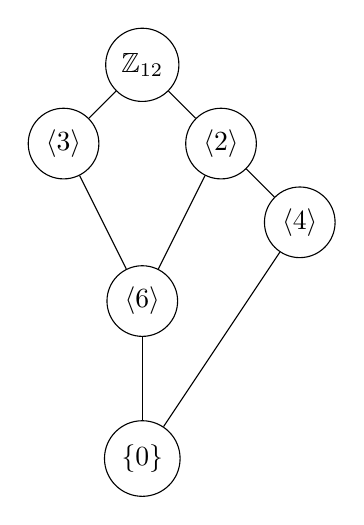
\begin{tikzpicture}
			\node[shape=circle,draw=black] (1) at (0,4) {$\Z_{12}$};
			\node[shape=circle,draw=black] (2) at (1,3) {$\langle 2\rangle$};
			\node[shape=circle,draw=black] (3) at (-1,3) {$\langle 3\rangle$};
			\node[shape=circle,draw=black] (4) at (2,2) {$\langle 4\rangle$};
			\node[shape=circle,draw=black] (6) at (0,1) {$\langle 6\rangle$};
			\node[shape=circle,draw=black] (12) at (0,-1) {$\{0\}$};
			
			\draw (1) -- (2);
			\draw (1) -- (3);
			\draw (2) -- (4);
			\draw (2) -- (6);
			\draw (3) -- (6);
			\draw (4) -- (12);
			\draw (6) -- (12);
		\end{tikzpicture}
	\end{myex}
	
	\section{Permutation groups}
	\begin{mydef}{Permutation group}{}
		Let $B=\{1, \dots, n\}$. A \underline{permutation} of $B$ is a bijection from $B$ to itself. That is to say, a function $\sigma:B\to B$ which is one-to-one and onto.
		
		Let $n\in\N$. Then, $S_n$ is the \underline{permutation group of order $n$}, the set of all permutations on $\{1, \dots, n\}$ with the operation being function composition.
		
		Elements $\sigma$ of $S_n$ can be denoted $\sigma=\begin{pmatrix}1&2&\dots&n\\\sigma(1)&\sigma(2)&\dots&\sigma(n)\end{pmatrix}$.
	\end{mydef}
	
	\begin{myrem}{Order of $S_n$}{}
		\begin{itemize}
			\item What is $|S_n|$? Let $\sigma\in S_n$. There are $n$ possibilities for $\sigma(1)$. Given $\sigma(1)$, there are $n-1$ possibilities for $\sigma(2)$, and so on. Thus, $|S_n|=n(n-1)(n-2)\dots1=n!$.
			
			\item $S_n$ is a non-abelian group. (Prove this!)
		\end{itemize}
	\end{myrem}
	
	\subsection{Cycle notation}
	\begin{mydef}{Cycles and transpositions}{}
		An expression of the form $(a_1\dots a_m)$ is a \underline{cycle length m}, and if $m=2$, a \underline{transposition}. For some $\sigma\in S_n$ we denote $\sigma=(a_1\dots a_m)$ to mean $\sigma(a_1)=a_2, \sigma(a_2)=a_3, \dots, \sigma(a_m)=a_1$.
	\end{mydef}
	
	\begin{myex}{Cycle notation for elements of $S_3$}{}
		Let $\sigma=\begin{pmatrix}1&2&3\\2&1&3\end{pmatrix}$. Then, $\sigma=(12)(3)$ since $\sigma(1)=2$ and $\sigma(2)=1$ and $\sigma(3)=3$.
		
		Let $\beta=\begin{pmatrix}1&2&3\\3&1&2\end{pmatrix}$. Then, $\beta=(132)=(321)=(213)$.
	\end{myex}
	
	\begin{myex}{Cycle notation for an element of $S_6$}{}
		Let $\sigma=\begin{pmatrix}1&2&3&4&5&6\\3&4&6&2&5&1\end{pmatrix}$. Then, $\sigma=(136)(24)=(24)(136)$.
	\end{myex}
	
	\begin{mythm}{Permutations are products of disjoint cycles}{6.6}
		Let $\sigma\in S_n$. Then, $\sigma$ can be written as a cycle or a product of disjoint cycles.
		\begin{proof}
			If $\sigma$ is a cycle we're done, so suppose it's not. Then, let $a_1\in\{1, \dots, n\}$ and $a_2=\sigma(a_1), \dots, a_k=\sigma(a_{k-1}), a_1=\sigma(a_k)$. This is always possible since $\{1, \dots, n\}$ is a finite set. Let $b_1\in\{1, \dots, n\}\setminus\{a_1, \dots, a_k\}$ and $b_2=\sigma(b_1), \dots, b_m=\sigma(b_{m-1}), b_1=\sigma(b_m)$. We claim the cycles $(a_1\dots a_k)$ and $(b_1\dots b_m)$ are disjoint.
			
			For contradiction suppose $a_i=b_j$ for some $i, j$. Then,
			\begin{align*}
				\sigma^{i-1}(a_1)&=\sigma^{j-1}(b_j)\\
				b_1&=\sigma^{j-1-i+1}(a_1)\in\{a_1, \dots, a_k\}
			\end{align*}
			which is impossible since $b_1\notin\{a_1, \dots, a_k\}$.
			
			Since $\{1, \dots, n\}$ is finite, this process stops eventually, and gives a representation of $\sigma$ as a product of disjoint cycles.
		\end{proof}
	\end{mythm}
	
	\begin{myex}{}{}
		Let $\tau=(124)$, $\sigma=(1235)$. What are $\tau\sigma$ and $\sigma\tau$ as a product of disjoint cycles?
		\begin{align*}
			\tau\sigma&=(124)(1235)=(14)(235)\\
			\sigma\tau&=(135)(24)
		\end{align*}
	\end{myex}
	
	\begin{myrem}{Aside}{}
		If $m\leq n$ then $S_m$ is ``isomorphic" to a subgroup of $S_n$. Section 8 introduces what it means for groups to be isomorphic.\\
		
		It is not technically true that $S_m\leq S_n$ because the elements of $S_m$ and elements of $S_n$ are functions on different sets so $S_m$ is not a subset of $S_n$.
	\end{myrem}
	
	\begin{mythm}{Disjoint cycles commute}{}
		Let $\sigma=(a_1\dots a_k)$, $\tau=(b_1\dots b_l)$ be disjoint cycles. Then $\sigma\tau=\tau\sigma$.
		\begin{proof}
			We know $\{1, \dots, n\}=\{a_1, \dots, a_k\}\cup\{b_1, \dots, b_l\}\cup\{c_1, \dots, c_m\}$
			
			where $\{c_1, \dots, c_m\}=\{1, \dots, n\}\setminus(\{a_1, \dots, a_k\}\cup\{b_1, \dots, b_l\})$. So,
			\begin{itemize}
				\item For all $i\in\{1, \dots, k\}$, we have $\tau(\sigma(a_i))=\tau(a_{i+1})=a_{i+1}=\sigma(a_i)=\sigma(\tau(a_i))$ since $\tau(a_i)=a_i$.
				\item For all $i\in\{1, \dots, l\}$, we have $\sigma(\tau(b_i))=\sigma(b_{i+1})=b_{i+1}=\tau(b_i)=\tau(\sigma(b_i))$ since $\sigma(b_i)=b_i$.
				\item For all $i\in\{1, \dots, m\}$, we have $\sigma(\tau(c_i))=\sigma(c_i)=c_i=\tau(c_i)=\tau(\sigma(c_i))$ since $\sigma(c_i)\tau(c_i)=c_i$.
			\end{itemize}
			 Therefore in all cases, $\sigma\tau=\tau\sigma$.
		\end{proof}
	\end{mythm}
	
	\begin{myrem}{}{}
		Let $\sigma$ be a $k$-cycle. Then $|\sigma|=k$.
	\end{myrem}
	
	\begin{mythm}{Order of a permutation}{}
		Let $\alpha\in S_n$. Then $|\alpha|$ is the least common multiple of the lengths of the disjoint cycles representing $\alpha$.
		\begin{proof}
			Let $\sigma, \tau\in S_n$ be disjoint cycles, with $\sigma$ being an $m$-cycle and $\tau$ being a $k$-cycle. Let $l=\text{lcm}(k, m)$. We claim $|\sigma\tau|=l$. Let $n=|\sigma\tau|$.
			
			Since $l=\text{lcm}(k, m)$, we have $k|l$ and $m|l$. So,
			\begin{align*}
				(\sigma\tau)^l&=\sigma^l\tau^l\\
				&=(\sigma^m)^t(\tau^k)^s
			\end{align*}
			for some $s, t\in\Z$. Thus,
			\begin{align*}
				\tau^k&=e=\sigma^m\\
				(\sigma\tau)^l&=e
			\end{align*}
			so $n\leq l$. Now, suppose $(\sigma\tau)^a=e$ for some $a\in\Z$. Then,
			\begin{align*}
				a&=q_1m+r_1=q_2k+r_2
			\end{align*}
			for some $q_1, q_2, r_1, r_2\in\Z$, $0\leq r_1<m$, $0\leq r_2<k$. So,
			\begin{align*}
				e=(\sigma\tau)^a&=\sigma^a\tau^a\\
				&=(\sigma^m)^{q_1}\sigma^{r_1}(\tau^k)^{q_2}\tau^{r_2}\\
				&=\sigma^{r_1}\tau^{r_2}\\
				\sigma^{-r_1}&=\tau^{r_2}
			\end{align*}
			But since $\sigma$ and $\tau$ are disjoint, the only way this can happen is if $\sigma^{-r_1}=\tau^{r_2}=e$. But $r_2<k$ so $r_2$ must be $0$. Similarly, $r_1=0$ as well. So, any integer $a$ such that $e=(\sigma\tau)^a$ is a multiple of both $k$ and $m$, and $l$ is the least such multiple by definition. Thus $|\sigma\tau|=l$.
		\end{proof}
	\end{mythm}
	
	\begin{myex}{}{}
		Find number of elements of order 3 in $S_7$.
		
		Suppose $\sigma\in S_7$ such that $|\sigma|=3$. So, $\sigma=(a_1a_2a_3)$ or $\sigma=(a_1a_2a_3)(a_4a_5a_6)$ where $a_i\neq a_j$ for all $i\neq j$. Thus, there are $\binom{7}{3}+\binom{7}{3}\binom{4}{3}$ such elements.
	\end{myex}
	
	\subsection{Transpositions and $A_n$}
	\begin{myrem}{}{}
		Recall that transpositions are 2-cycles. They are special because they generate $S_n$.
	\end{myrem}
	
	\begin{myex}{}{}
		Consider $(1234)\in S_n$. Now, $(1234)=(14)(13)(12)$.
	\end{myex}
	
	\begin{mythm}{}{6.15}
		Let $\sigma=(a_1\dots a_m)$ be a cycle of length $m\geq2$. Then $m$ can be written as a product of transpositions.
		\begin{proof}
		Only a proof sketch is given.
			\begin{align*}
				(a_1\dots a_m)&=(a_1a_m)(a_1a_{m-1})\dots(a_1a_2)
			\end{align*}
		\end{proof}
	\end{mythm}
	
	\begin{mycor}{}{}
		Let $\sigma\in S_n$. Then $\sigma$ can be written as a product of transpositions.
		\begin{proof}
			Directly follows from theorems \ref{th:6.6} and \ref{th:6.15}.
		\end{proof}
	\end{mycor}
	
	\begin{myex}{}{}
		Consider $(123)\in S_4$.
		\begin{align*}
			(123)&=(13)(12)\\
			&=(13)(24)(13)(24)(13)(12)
		\end{align*}
	\end{myex}
	
	\begin{mylem}{}{IdIsEven}
		Let $e$ be the identity in $S_n$. If $e=\beta_1\dots\beta_k$ for transpositions $\beta_1, \dots, \beta_k$, then $k$ is even.
		\begin{proof}
			Shamelessly stolen from the textbook.\\\includegraphics[scale=.7]{textproof1.png}
		\end{proof}
	\end{mylem}
	
	\begin{mythm}{}{EvenIsEven}
		Let $\sigma\in S_n$. If $\sigma=\beta_1\dots\beta_m=\gamma_1\dots\gamma_k$ for transpositions $\beta_1, \dots, \beta_m, \gamma_1, \dots, \gamma_k$, then $m\equiv k\mod2$.
		\begin{proof}
			Let $\beta_i=(a_ib_i)$ and $\gamma=(c_jd_j)$ for $i=1\dots m$, $j=1\dots k$. Then,
			\begin{align*}
				\sigma&=(a_1b_1)\dots(a_mb_m)=(c_1d_1)\dots(c_kd_k)\\
				\sigma\sigma\inv=e&=(c_1d_1)\dots(c_kd_k)(a_mb_m)\inv\dots(a_1b_1)\inv\\
				&=(c_1d_1)\dots(c_kd_k)(a_mb_m)\dots(a_1b_1)\\
			\end{align*}
			Thus by Lemma \ref{le:IdIsEven} we know $k+m$ is even, so $k$ and $m$ must have the same parity.
		\end{proof}
	\end{mythm}
	
	\begin{mydef}{Even and Odd permutations}{}
		Let $\sigma\in S_n$. If $\sigma$ is a product of an even number of permutations, then $\sigma$ is \underline{even}. Otherwise $\sigma$ is \underline{odd}.\\
		
		We define $A_n:=\{\sigma\in S_n:\sigma\text{ is even}\}$, and this is called the \underline{alternating group of order $n$}.
	\end{mydef}
	
	\begin{myex}{}{}
		In $S_3$ $e, (123), (132)$ are even while $(12), (13), (23)$ are odd.
	\end{myex}
	
	\begin{mythm}{Alternating groups are groups}{}
		$A_n\leq S_n$.
		\begin{proof}
			We know $e\in A_n$ so $A_n\neq\emptyset$. Let $\sigma, \tau\in A_n$. Then,
			\begin{align*}
				\sigma&=\sigma_1\dots\sigma_{2n}\\
				\tau&=\tau_1\dots\tau_{2k}
			\end{align*}
			for integers $k, n$ and transpositions $\sigma_1, \dots, \sigma_{2n}, \tau_1, \dots, \tau_{2k}$. So, $\sigma\tau\inv=\sigma_1\dots\sigma_{2n}\tau_{2k}\dots\tau_{2k}$ is even since it is the product of $2k+2n=2(k+n)$ transpositions. Hence $A_n\leq S_n$ by one-step-test.
		\end{proof}
	\end{mythm}
	
	\section{Normal subgroups}
	\subsection{Introduction}
	
	\begin{myrem}{}{}
		Let $G$ be a group, and $H\leq G$. We know given $a\in G$, the left coset $aH$ does not always equal the right coset $Ha$. Subgroups whose left cosets are equal to their right cosets are given a special name.
	\end{myrem}
	
	\begin{mydef}{Normal subgroup}{}
		Let $G$ be a group, and $H\leq G$. $H$ is \underline{normal} if for all $a\in G$ we have $aH=Ha$. We denote this by $H\lhd G$.
	\end{mydef}
	
	\begin{myrem}{}{}
		If $H\lhd G$, we have $ah=h'a$ for all $a\in G$ and $h, h'\in H$. However $ah$ is not necessarily equal to $ha$.
	\end{myrem}
	
	\begin{mythm}{}{}
		Let $G$ be a group, and $H\leq G$. Then $H\lhd G$ iff for all $a\in G$, $aHa\inv\subseteq H$.
		\begin{proof}
			$(\Longrightarrow)$ Suppose $H\lhd G$. Let $a\in G$. Then
			\begin{align*}
				aHa\inv&=Haa\inv\\
				&=He\\
				&=H\subseteq H
			\end{align*}
			
			$(\Longleftarrow)$ Suppose for all $a\in G$, $aHa\inv\subseteq H$. Then,
			\begin{align*}
				aH\subseteq Ha
			\end{align*}
			by right cancellation. Also since $a\inv\in G$, we have $a\inv Ha\subseteq H$ so
			\begin{align*}
				Ha\subseteq H
			\end{align*}
			Thus $aH=Ha$ and by definition $H\lhd G$.
		\end{proof}
	\end{mythm}
	
	\begin{myex}{Abelian groups have only normal subgroups}{}
		Let $G$ be abelian. Then, all subgroups of $G$ are normal.
		\begin{proof}
			Let $H\leq G$. Then for all $a\in G$ and $h\in H$, $ah=ha$, so $aH=Ha$.
		\end{proof}
	\end{myex}
	
	\begin{myex}{Center of group is normal}{}
		$Z(G)\lhd G$.
		\begin{proof}
			Let $a\in G$. Then, $aZ(G)a\inv=aa\inv Z(G)=Z(G)\subseteq Z(G)$.
		\end{proof}
	\end{myex}
	
	\begin{myex}{Alternating group is normal subgroup of symmetric group}{}
		$A_n\lhd S_n$.
		\begin{proof}
			Let $\sigma=\sigma_1\dots\sigma_k\in S_n$, $\alpha=\alpha_1\dots\alpha_{2q}\in A_n$ where $n, k, q\in\Z$ and $\sigma_1, \dots, \sigma_{k},$ $\alpha_1, \dots, \alpha_{2q}$ are transpositions. Then, $\sigma\alpha\sigma\inv$ is a product of $k+2q+k$ transpositions, which is an even number.
		\end{proof}
	\end{myex}
	
	\begin{myex}{}{}
		Consider $3\Z\leq \Z$. Since $\Z$ is abelian, $3\Z\lhd\Z$. Consider the cosets of $3\Z$ in $\Z$.
		\begin{align*}
			0+3\Z&=\{\dots, -3, 0, 3, \dots\}\\
			1+3\Z&=\{\dots, -2, 1, 4, \dots\}\\
			2+3\Z&=\{\dots, -1, 2, 5, \dots\}
		\end{align*}
		Let $F=\{3\Z, 1+3\Z, 2+3\Z\}$. Define $(a+3\Z)+(b+3\Z)=(a+b)+3\Z$ where $a, b\in\Z_3$. Note that $F$ ``looks like" $\Z_3$.
	\end{myex}
	
	\subsection{Quotient groups}
	\begin{mythm}{Quotient groups are groups}{}
		Let $G$ be a group, and $H\leq G$. Then, $H\lhd G$ iff $G/H:=\{gH:g\in G\}$ is a group under operation $(aH)(bH):=(ab)H$ for $a, b\in G$.
		
		The group $G/H$ is called the \underline{quotient group of G by H}, or \underline{factor group}.
		\begin{proof}
			$(\Longrightarrow)$ Suppose $H\lhd G$. First, check the operation is well-defined. We need to show if $aH=a'H$ and $bH=b'H$ for some $a, a', b, b'\in G$ then $(aH)(bH)=(ab)H=(a'b')H=(a'H)(b'H)$.
			
			\begin{align*}
				(aH)(bH)&=(ab)H\\
				&=a(bH)\\
				&=a(b'H)\\
				&=a(Hb')\\
				&=(aH)b'\\
				&=(a'H)b'\\
				&=a'(Hb')\\
				&=a'b'H\\
				&=(a'H)(b'H)
			\end{align*}
			Thus, $(aH)(bH)=(a'h_1H)(b'h_2H)=(a'H)(b'H)$ so the operation is well-defined.\\
			
			\textbf{(Identity.)} $eH=H$ is the identity element since $(eH)(gH)=gH=(gH)(eH)$ for all $g\in G$.\\
			
			\textbf{(Inverses.)} Let $a\in G$. Then, $(aH)(a\inv H)=eH=(a\inv H)(aH)$.\\
			
			\textbf{(Closure.)} Follows from closure of $G$.\\
			
			\textbf{(Associativity.)} Follows from associativity of $G$.
			
			So $G/H$ is a group.
			
			$(\Longleftarrow)$ Suppose $G/H$ is a group, and therefore its operation is well-defined. Let $g\in G$. It will be shown that $gHg\inv\subseteq H$.
			
			Let $h\in H$. Then,
			\begin{align*}
				g\inv H&=(eg\inv)H\\
				&=eHg\inv H\\
				&=hHg\inv H\\
				&=(hg\inv)H\\
				H&=(ghg\inv)H
			\end{align*}
			Therefore $ghg\inv\in H$ and hence $gHg\inv\subseteq H$ so $H\lhd G$.
		\end{proof}
	\end{mythm}
	
	\begin{myrem}{Aside}{}
		For this operation to be well defined it is not sufficient to show if $aH=a'H$ and $bH=b'H$ then $(aH)(bH)=(a'H)(b'H)$. One also needs to show $(ab)H=(a'b')H$. These notes present a correct proof.
	\end{myrem}
	
	\begin{mycor}{}{}
		Let $G$ be a group, and $H\lhd G$. Then, $|G/H|=|G:H|=\frac{|G|}{|H|}$.
	\end{mycor}
	
	\begin{myex}{}{}
		$|\Z_{10}/\langle 6\rangle|=\frac{|\Z_{10}|}{|\langle 6\rangle|}=\frac{10}{5}=2$
		
		We can therefore deduce that $\Z_{10}/\langle 6\rangle=\{\langle 6\rangle, 1+\langle 6\rangle\}$
	\end{myex}
	
	\begin{mythm}{$G/Z$ theorem}{gz}
		Let $G$ be a group. If $G/Z(G)$ is cyclic, then $G$ is abelian.
		\begin{proof}
			Let $x, y\in G$. Since $G/Z(G)$ is cyclic, we have $\langle [a]\rangle:=\langle aZ(G)\rangle=G/Z(G)$ for some $a\in G$. So,
			\begin{align*}
				xZ(G)&=a^mZ(G)\\
				yZ(G)&=a^nZ(G)
			\end{align*}
			for some $m, n\in\Z$. Therefore for some $z_1, z_1', z_2, z_2'\in Z(G)$ we have
			\begin{align*}
				xz_1&=a^mz_1'\\
				x&=a^mz_1'z_1\inv
			\end{align*}
			So $x=a^mz_x$ for some $z_x\in Z(G)$. Similarly $y=a^nz_y$ for some $z_y\in Z(G)$. Thus,
			\begin{align*}
				xy&=a^mz_xa^nz_y\\
				&=z_xa^{m+n}z_y\\
				&=z_xa^na^mz_y\\
				&=a^nz_ya^mz_x\\
				&=yx
			\end{align*}
			since $z_x, z_y$ commute with all elements of $G$. Therefore $G$ is abelian.
		\end{proof}
	\end{mythm}
	
	\begin{mythm}{Cauchy's theorem for abelian groups}{cauchy1}
		Let $G$ be a finite abelian group, with $|G|=n$. If $p$ is a prime number which is a factor of $n$, then there exists $H\leq G$ such that $|H|=p$.
		
		\begin{proof}
			(The general, non-abelian case is proven in theorem \ref{th:cauchy}.)
			
			By strong induction on $n$.\\
			
			\textbf{Base case: }The statement is trivially true for the groups of order 1 and 2.\\
			
			\textbf{Inductive step: }Suppose the statement is true for all groups of order less than $n$. Let $g\in G$ such that $g\neq e$ and let $|g|=m=qs$ for some $q, s\in\Z$ with $q$ prime. Let $a=g^s$. So, $|a|=q$.\\
			
			If $q=p$ then $\langle a\rangle\leq G$ with $|\langle a\rangle|=p$ so we're done.\\
			
			Since $G$ is assumed to be abelian, we know $\langle a\rangle\lhd G$. Then, $|G/\langle a\rangle|=\frac{n}{q}$. We also know $\frac{n}{q}<n$ and $p$ is a factor of $\frac{n}{q}$. Therefore by inductive hypothesis, $G/\langle a\rangle$ has a subgroup $H$ such that $|H|=p$. So, $H$ is cyclic: there exists $y\in G$ such that $H=\langle [y]\rangle$ where $[y]=y\langle a\rangle$.\\
			
			We know that $[y]^p=[e]=\langle a\rangle$. Therefore $y^p\in\langle a\rangle$. So $y^p=a^k$ for some $k\in\Z$, and
			\begin{align*}
				y^{pq}&=a^{kq}\\&=(a^q)^k\\
				&=e
			\end{align*}
			Thus the possible orders of $y$ are $1, p, q, pq$ by Lagrange's theorem.
			\begin{itemize}
				\item If $|y|=1$ then $H$ is a trivial subgroup, which contradicts $|H|=p$, so this is impossible.
				\item If $|y|=p$ then $|\langle y\rangle|=p$ as desired.
				\item If $|y|=q$ then $[y]^q=y^qH=eH=H=[y]^p$ since $|[y]|=p$. So, $p$ is a proper factor of $q$, which contradicts $p$ and $q$ being prime.
				\item If $|y|=pq$ then $|y^q|=p$ so $|\langle y^q\rangle|=p$ as desired.
			\end{itemize}
		\end{proof}
	\end{mythm}
	
	\section{Isomorphisms and homomorphisms}
	\subsection{Isomorphisms}
	\begin{myrem}{$\Z_2$ and $\Z_6^*$ have the same structure}{}
		Consider the Cayley tables of the groups $\Z_2$ and $\Z_6^*$.
		\begin{align*}
			\begin{array}{c | cc}
			+ & 0 & 1\\
			\hline
			0     & 0 & 1 \\
			1     & 1 & 0 \\
			\end{array}\\
			\begin{array}{c | cc}
			\cdot & 1 & 5\\
			\hline
			1     & 1 & 5 \\
			5     & 5 & 1 \\
			\end{array}
		\end{align*}
		Clearly, one can simply relabel the elements of one group as follows, and obtain the other group: $0\leftrightarrow1, 1\leftrightarrow5$.
	\end{myrem}
	
	\begin{mydef}{Isomorphism}{}
		Let $G$, $G'$ be groups. Then a function $\phi:G\to G'$ is an \underline{isomorphism} if:
		\begin{enumerate}
			\item $\phi$ is one-to-one.
			\item $\phi$ is onto.
			\item $\phi$ preserves group operation. That is, for all $a, b\in G$ we have $\phi(ab)=\phi(a)\phi(b)$.
		\end{enumerate}
		
		If there exists an isomorphism between $G$ and $G'$ then we say $G$ is \underline{isomorphic to} $G'$, with notation $G\cong G'$. If $G$ is not isomorphic to $G'$ we say $G\ncong G'$.
	\end{mydef}
	
	\begin{myrem}{}{}
		Isomorphisms represent ``equality" of groups up to relabelling the elements.
	\end{myrem}
	
	\begin{myex}{}{}
		All infinite cyclic groups are isomorphic to $\Z$.
		\begin{proof}
			Let $G=\langle a\rangle$ be an infinite cyclic group. So, for all $g\in G$ we have $g=a^k$ for some $k\in\Z$. Define $\phi:G\to\Z$ by $\phi(a^n)=n$. Then,\\
			
			\textbf{(One-to-one.)} Suppose $\phi(g)=\phi(g')$ for $g, g'\in G$. Therefore, $g=a^m, g'=a^{m'}$ for $m, m'\in\Z$. Thus,
				
			\begin{align*}
				\phi(a^m)&=\phi(a^{m'})\\
				m&=m'\\
				a^m&=a^{m'}\\
				g&=g'
			\end{align*}
			So $\phi$ is one-to-one.\\
			
			\textbf{(Onto.)} Let $n\in\Z$. Then $\phi(a^n)=n$ so $\phi$ is onto.\\
			
			\textbf{(Preserves group operation.)} We have $\phi(gg')=\phi(a^ma^{m'})=\phi(a^{m+m'})=m+m'$ so $\phi$ preserves group operation.
		\end{proof}
	\end{myex}
	
	\begin{myex}{}{}
		Let $G$ be a finite cyclic group of order $n$. Then $G\cong\Z_n$.
		\begin{proof}
			Let $G=\langle a\rangle$. Then, for all $g\in G$ we have $g=a^k$ for some $k\in\Z$. Define $\phi:G\to\Z_n$ by $\phi(g)=\phi(a^k)=k$. We can show $\phi$ is an isomorphism by an argument similar to that in the previous example.
		\end{proof}
	\end{myex}
	
	\begin{mythm}{Properties of isomorphisms}{}
		Let $\phi:G\to H$ be an isomorphism of groups $G, H$. Let $e_G\in G, e_H\in H$ be the identities of $G$ and $H$ respectively. Then,
		\begin{enumerate}
			\item $\phi(e_G)=e_H$
			\item For any $n\in\Z$, we have $\phi(a^n)=(\phi(a))^n$ where $a\in G$.
			\item If $G=\langle a\rangle$ then $H=\langle \phi(a)\rangle$.
			\item For all $a\in G$ we have $|a|=|\phi(a)|$.
			\item If $G$ is finite then $|G|=|H|$.
		\end{enumerate}
		\begin{proof}~\\
			\begin{enumerate}
				\item We have $\phi(e_G)\phi(g)=\phi(e_Gg)=\phi(g)$ for all $g\in G$. Therefore $\phi(e_G)$ must be the identity element.
				\item Follows by induction on $n$ since $\phi$ preserves group operations.
				\item Follows from (2).
				\item Follows from (2).
				\item Follows from $\phi$ being a bijection.
			\end{enumerate}
		\end{proof}
	\end{mythm}
	
	\begin{myex}{Non-example of isomorphism}{}
		Let $G$ be a group and $g\in G$. Define $\phi_g:G\to G$ by $\phi_g(x)=gx$ for all $x\in G$. Then $\phi_g$ is a bijection, but not necessarily an isomorphism, since $\phi_G(xy)=gxy\neq gxgy$ in general.
	\end{myex}
	
	\begin{mythm}{Cayley's theorem}{cayleythm}
		Let $G$ be a group. Then $G$ is isomorphic to a group of permutations.
		\begin{proof}
			Define $\overline{G}:=\{\phi_g:g\in G\}$. First it will be shown that $\overline{G}$ is a group under the operation of composition. Note that $\overline{G}$ is a set of bijections of $G$.\\
			
			\textbf{(Closure.)} Let $\phi_{g_1}, \phi_{g_2}\in\overline{G}$. Then $(\phi_{g_1}\circ\phi_{g_2})(x)=\phi_{g_1}(\phi_{g_2}(x))=g_1g_2x=\phi_{g_1g_2}$ for all $x\in G$ so $\overline{G}$ is closed under composition.\\
			
			\textbf{(Associativity.)} Let $\phi_{g_1}, \phi_{g_2}, \phi_{g_3}\in\overline{G}$. Then, $(\phi_{g_1}\circ\phi_{g_2})\circ\phi_{g_3}(x)=\phi_{g_1}(\phi_{g_2}(\phi_{g_3}(x)))=\phi_{g_1}\circ(\phi_{g_2}\circ\phi_{g_3})(x)$ for all $x\in G$ so composition is associative.\\
			
			\textbf{(Identity.)} $(\phi_e\circ\phi_g)(x)=\phi_e(\phi_g(x))=egx=gx=gex=\phi_g(\phi_e(x))=(\phi_g\circ\phi_e)(x)$ for all $g, x\in G$. Therefore $\phi_e$, the identity mapping, is the identity element in $\overline{G}$.\\
			
			\textbf{(Inverses.)} For all $\phi_g\in\overline{G}$ we have $(\phi_{g\inv}\circ\phi_g)(x)=gg\inv x=x=g\inv gx=(\phi_g\circ\phi_{g\inv})(x)$ so all elements of $\overline{G}$ have an inverse.\\
			
			So $\overline{G}$ is a group. Now it will be shown that $G\cong\overline{G}$. Define $\psi:\overline{G}\to G$ by $\psi(\phi_g)=g$.\\
			
			\textbf{(One-to-one.)} Let $\phi_{g_1}, \phi_{g_2}\in\overline{G}$ such that $\psi(\phi_{g_1})=\psi(\phi_{g_2})$. Then by definition $g_1=g_2$ so $\phi_{g_1}=\phi_{g_2}$. Hence $\psi$ is one-to-one.\\
			
			\textbf{(Onto.)} Let $g\in G$. Then $\psi(\phi_g)=g$ so $\psi$ is onto.\\
			
			\textbf{(Preserves group operation.)} Let $\phi_{g_1}, \phi_{g_2}\in\overline{G}$ and $x\in G$. Then
			\begin{align*}
				\psi(\phi_{g_1}\circ\phi_{g_2})x&=g_1g_2x\\
				&=\psi(\phi_{g_1})\psi(\phi_{g_2})x
			\end{align*}
			
			Therefore $G\cong\overline{G}$.
		\end{proof}
	\end{mythm}
	
	\subsection{Homomorphisms}
	
	\begin{mydef}{Homomorphism}{}
		Let $G, H$ be groups. A map $\phi:G\to H$ is a \underline{homomorphism} if $\phi$ preserves the group operation. That is, if
		\begin{align*}
			\phi(g_1g_2)&=\phi(g_1)\phi(g_2)
		\end{align*}
		for all $g_1, g_2\in G$.
	\end{mydef}
	
	\begin{myex}{}{}
		Define $\phi:\Z\to\Z_n$ by $\phi(k)=k\mod n$. Let $k, l\in\Z$. Then,
		\begin{align*}
			\phi(k+l)&=k+l\mod n\\
			&=k\mod n+l\mod n\\
			&=\phi(k)+\phi(l)
		\end{align*}
		so $\phi$ is a homomorphism.
	\end{myex}
	
	\begin{myex}{Trivial homomorphism}{}
		Define $\phi:G\to H$ by $\phi(g)=e$ for all $g\in G$. Then $G$ is a homomorphism.\\
		
		This shows there is a homomorphism between any groups $G$ and $H$, so it makes no sense to call two groups ``homomorphic".
	\end{myex}
	
	\begin{myex}{}{}
		Recall, $\R^*=\{x\in\R:x\neq0\}$ with multiplication is a group. Now, $\varphi:\R^*\to\R^*$ defined by $x\mapsto|x|$ is a homomorphism since $|xy|=|x||y|$ for all $x, y\in\R^*$.
	\end{myex}
	
	\begin{myex}{}{}
		Recall the set of invertible real matrices of size $n$, $GL_n(\R)$. Now, $\varphi:GL_n(\R)\to\R^*$ defined by $A\mapsto\det(A)$ is a homomorphism, since $\det(AB)=\det(A)\det(B)$ for all $A, B\in GL_n(\R)$.
	\end{myex}
	
	\begin{myex}{Non-example of a homomorphism}{}
		Consider $\phi:(\R, +)\to(\R, +)$ defined by $x\mapsto x^2$. This is not a homomorphism since $\phi(1+1)=4\neq2=\phi(1)+\phi(1)$.
	\end{myex}
	
	\begin{myex}{}{}
		Define $\varphi:\Z_2\to\Z_2$ by $x\mapsto x^2$. This is a homomorphism because
		\begin{align*}
			\varphi(x+y)&=x^2+2xy+y^2\\
			&=x^2+y^2\\
			&=\varphi(x)+\varphi(y)
		\end{align*}
		since $2xy=0$ for all $x, y\in\Z_2$.
	\end{myex}
	
	\begin{mydef}{Kernel and Image}{}
		Let $\varphi:G\to H$ be a homomorphism between groups $G$, $H$.
		
		The \underline{kernel} of $\varphi$ is $\ker\varphi:=\{g\in G:\varphi(g)=e\}$ where $e$ is the identity in $H$.
		
		The \underline{image} of $\varphi$ is $\Im\varphi:=\{\varphi(g):g\in G\}$.
	\end{mydef}
	
	\begin{myex}{}{}
		If $\varphi$ is the trivial homomorphism then $\ker\varphi=G$ and $\Im\varphi=\{e\}$.
	\end{myex}
	
	\begin{myex}{}{}
		If $\varphi:\Z\to\Z_n$ is defined by $\varphi(k)=k\mod n$ then $\ker\varphi=n\Z$ and $\Im\varphi=Z_n$.
	\end{myex}
	
	\begin{myex}{}{}
		If $\varphi:\R^*\to\R^*$ is defined by $\varphi(x)=|x|$ then $\ker\varphi=\{-1, 1\}$ and
		
		$\Im\varphi=\{x\in\R:x>0\}=:\R^+$.
	\end{myex}
	
	\begin{myex}{}{}
		If $\varphi:GL_n(\R)\to\R^*$ is defined by $\varphi(A)=\det(A)$, then $\ker\varphi=\{A\in GL_n(\R):\det(A)=1\}$ and $\Im\varphi=\R^*$.
	\end{myex}
	
	\begin{mythm}{}{}
		Let $\varphi:G\to H$ be a homomorphism from $G$ to $H$. Then:
		\begin{enumerate}
			\item $\varphi(e_G)=e_H$ where $e_G, e_H$ are the identity elements in $G$ and $H$ respectively.
			\item For all $a\in G$ we have $\varphi(a\inv)=\varphi(a)\inv$.
			\item $\Im\varphi\leq H$
			\item $\ker\varphi\leq G$
			\item $\ker\varphi\lhd G$
		\end{enumerate}
		\begin{proof}~\\
			\begin{enumerate}
				\item Let $g\in G$. Then $\varphi(g)=\varphi(e_Gg)=\varphi(e_G)\varphi(g)$ so $\varphi(e_G)$ must be the identity in $H$.
				\item We have $\varphi(e_G)=\varphi(aa\inv)=\varphi(a)\varphi(a\inv)=e_H$ so $\varphi(a\inv)=\varphi(a)\inv$.
				\item Notice $\Im\varphi\neq\emptyset$ since $e_H\in\Im\varphi$. Let $a, b\in\Im\varphi$. Then $\varphi(g_1)=a$ and $\varphi(g_2)=b$ for some $g_1, g_2\in G$. So,
				\begin{align*}
					ab\inv&=\varphi(g_1)\varphi(g_2)\inv\\
					&=\varphi(g_1)\varphi(g_2\inv)\\
					&=\varphi(g_1g_2\inv)
				\end{align*}
				Since $g_1g_2\inv\in G$ we have $ab\inv\in\Im\varphi$ so by one-step test, $\Im\varphi\leq H$.
				\item Notice $\ker\varphi\neq\emptyset$ since $\varphi(e_G)=e_H$ so $e_G\in\ker\varphi$. Let $a, b\in\ker\varphi$. Then,
				\begin{align*}
					\varphi(ab\inv)&=\varphi(a)\varphi(b\inv)\\
					&=\varphi(a)\varphi(b)\inv\\
					&=e_He_H\inv\\
					&=e_H
				\end{align*}
				Therefore, $ab\inv\in\ker\varphi$ so by one-step test, $\ker\varphi\leq G$.
				\item It will be shown that for all $a\in G$ we have $a(\ker\varphi)a\inv\subseteq\ker\varphi$. Let $a\in G$, $g\in\ker\varphi$. Then,
				\begin{align*}
					\varphi(aga\inv)&=\varphi(a)\varphi(g)\varphi(a\inv)\\
					&=\varphi(a)e_H\varphi(a)\inv\\
					&=e_H
				\end{align*}
				Therefore $a(\ker\varphi)a\inv\subseteq\ker\varphi$ so $\ker\varphi\lhd G$.
			\end{enumerate}
		\end{proof}
	\end{mythm}
	
	\subsection{Automorphisms}
	
	\begin{mydef}{Automorphism}{}
		Let $G$ be a group. An isomorphism $\varphi:G\to G$ is called an \underline{automorphism} and the set of automorphisms of $G$ is denoted $Aut(G)$.
		
		A mapping $\phi_a:G\to G$ defined by $g\mapsto aga\inv$ for some $a\in G$ is called an \underline{inner automorphism} and the set of inner automorphisms of $G$ is denoted $Inn(G)$.
	\end{mydef}
	
	\begin{myex}{Identity automorphism}{}
		For any groups $G$ the identity mapping $id:G\to G$ defined by $g\mapsto g$ is an automorphism.
	\end{myex}
	
	\begin{myex}{Conjugation automorphism}{}
		The mapping $\varphi:\C\to\C$ defined by $a+bi\mapsto a-bi$ is an automorphism on $\C$.
	\end{myex}
	
	\begin{mythm}{}{}
		Let $G$ be a group.
		\begin{enumerate}
			\item $Aut(G)$ is a group under composition.
			\item $Inn(G)\leq Aut(G)$
			\item $Inn(G)\lhd Aut(G)$
		\end{enumerate}
	\end{mythm}
	
	\begin{myrem}{}{}
		In $Aut(G)$ the identity is the identity mapping and the inverse of an element is the element's inverse function (which exists since all elements of $Aut(G)$ are bijections).
	\end{myrem}
	
	\begin{myex}{}{}
		Find $Inn(D_4)$.\\
		
		Recall, $D_4=\{e, R, R^2, R^3, H, V, D, D'\}$. Notice that if $g\in Z(D_4)$ then $\phi_g(x)=x$ for all $x\in D_4$, meaning $\phi_g=id$. Also recall that $Z(D_4)=\{e, R^2\}$. Let $x\in D_4$. Then,
		\begin{align*}
			\phi_{R^3}(x)=R^3x(R^3)\inv\\
			&=(RR^2)x(RR^2)\inv\\
			&=R(R^2xR^2)R\inv\\
			&=RxR\inv\\
			&=\phi_R(x)
		\end{align*}
		So $\phi_{R^3}=\phi_R$. Now, $VR^2=H$ so
		\begin{align*}
			\phi_H(x)&=HxH\\
			&=(VR^2)x(VR^2)\inv\\
			&=V(R^2xR^2)V\\
			&=VxV\\
			&=\phi_V(x)
		\end{align*}
		So $\phi_V=\phi_H$. Similarly $\phi_D=\phi_{D'}$. So, $Inn(D_4)=\{id, \phi_R, \phi_H, \phi_D\}$.\\
		
		Now, $D_4/Z(D_4)=\{[e], [R], [H], [D]\}$. It turns out that $D_4/Z(D_4)\cong Inn(D_4)$.
	\end{myex}
	
	\begin{myex}{Automorphisms on finite cyclic groups}{}
		What is $Aut(\Z_n)$?\\
		
		Let $\phi:\Z_n\to\Z_n$ be an isomorphism. Since $\Z_n=\langle 1\rangle$, we can determine $\phi$ if we know $\phi(1)$. Also, since $\phi$ is an isomorphism, $\Z_n=\langle\phi(1)\rangle$. The set of generators of $\Z_n$ is $\Z_n^*$, so $\phi(1)\in\{m\in\Z_n:\gcd(m, n)=1\}$.
	\end{myex}
	
	\begin{mythm}{}{}
		$Aut(\Z_n)\cong\Z_n^*$.
		\begin{proof}
			Define $F:Aut(\Z_n)\to\Z_n^*$ by $\phi\mapsto\phi(1)$. $F$ is well-defined since $F(\phi)\in\Z_n^*$ for all $\phi\in Aut(\Z_n)$. It will be shown that $F$ is an isomorphism.\\
			
			\textbf{(One-to-one.)} Let $\phi_1, \phi_2\in Aut(\Z_n)$ such that $F(\phi_1)=F(\phi_2)$. Then for all $x\in\Z_n$,
			\begin{align*}
				\phi_1(x)&=\phi_1(\underbrace{1+\dots+1}_x)\\
				&=\underbrace{\phi_1(1)+\dots+\phi_1(1)}_x\\
				&=\underbrace{\phi_2(1)+\dots+\phi_2(1)}_x\\
				&=\phi_2(\underbrace{1+\dots+1}_x)\\
				&=\phi_2(x)
			\end{align*}
			so $\phi_1=\phi_2$.\\
			
			\textbf{(Onto.)} Let $k\in\Z_n^*$. Then the function $\phi\in Aut(\Z_n)$ defined by $\phi(1)=k$ is such that $F(\phi)=k$, so $F$ is onto.\\
			
			\textbf{(Homomorphism.)} Let $\phi_1, \phi_2\in Aut(\Z_n)$. Then,
			\begin{align*}
				F(\phi_1\circ\phi_2)&=(\phi_1\circ\phi_2)(1)\\
				&=\phi_1(\phi_2(1))\\
				&=\phi_1(\underbrace{1+\dots+1}_{\phi_2(1)})\\
				&=\underbrace{\phi_1(1)+\dots+\phi_1(1)}_{\phi_2(1)}\\
				&=\phi_1(1)\phi_2(1)\\
				&=F(\phi_1)F(\phi_2)
			\end{align*}
			
			Therefore $Aut(\Z_n)\cong\Z_n^*$.
		\end{proof}
	\end{mythm}
	
	\begin{myex}{}{}
		Let $p$ be prime. Then, $|Aut(\Z_p)|=p-1$.
	\end{myex}
	
	\subsection{First isomorphism theorem}
	
	\begin{myex}{}{}
		Recall $\ker\phi$ is a normal subgroup for any homomorphism $\phi$. In particular, $A_n\lhd S_n$. Notice that $|S_n/A_n|=2$ so $S_n/A_n\cong\Z_2$.
	\end{myex}
	
	\begin{mythm}{First isomorphism theorem}{fit}
		Let $\phi:G\to H$ be a homomorphism. Then, $G/\ker\phi\cong\Im\phi$.
		\begin{proof}
			Let $K=\ker\phi$. Define $\psi:G/K\to\Im\phi$ by $gK=[g]\mapsto\phi(g)$. It will be shown that this is an isomorphism.
			
			\textbf{(Well-defined.)} Let $[g_1]=[g_2]$. Then, $g_1=g_2k$ for some $k\in K$.
			\begin{align*}
				\psi([g_1])&=\phi(g_1)\\
				&=\phi(g_2k)\\
				&=\phi(g_2)\phi(k)\\
				&=\phi(g_2)\\
				&=\psi([g_2])
			\end{align*}
			so $[g_1]=[g_2]\Longrightarrow\psi([g_1])=\psi([g_2])$ and thus $\psi$ is well-defined.\\
			
			\textbf{(One-to-one.)} Suppose $[g_1], [g_2]\in G/K$ such that $\psi([g_1])=\psi([g_2])$. Then,
			\begin{align*}
				\phi(g_1)&=\phi(g_2)\\
				\phi(g_1)\phi(g_2)\inv&=e\\
				\phi(g_1g_2\inv&=e\\
				\therefore g_1, g_2\inv&\in K\\
				\therefore g_1&=g_2k\text{ for some }k\in K\\
				\therefore g_1&\in g_2K\\
				\therefore [g_1]&=[g_2]
			\end{align*}
			so $\psi$ is one-to-one.\\
			
			\textbf{(Onto.)} Let $h\in\Im\phi$. Since $\phi$ is surjective, there exists $g\in G$ such that $\phi(g)=h$. So, $\psi([g])=h$ and $\psi$ is onto.\\
			
			\textbf{(Homomorphism.)} Let $[g_1], [g_2]\in G/K$. Then,
			\begin{align*}
				\psi([g_1][g_2])&=\psi([g_1g_2])\\
				&=\phi(g_1g_2)\\
				&=\phi(g_1)\phi(g_2)\\
				&=\psi([g_1])\psi([g_2])
			\end{align*}
			so $\psi$ is a homomorphism and hence an isomorphism.
		\end{proof}
	\end{mythm}
	
	\begin{mycor}{}{}
		\begin{enumerate}
			\item Let $\phi:G\to H$ be a homomorphism, with $G, H$ both finite. Then $|\Im\phi|$ divides both $|G|$ and $|H|$.
			
			\item Let $G$ be a group. Then, $G/Z(G)\cong Inn(G)$.
		\end{enumerate}
		\begin{proof}~\\
			\begin{enumerate}
				\item We know $\Im\phi\leq H$ so $|\Im\phi|$ divides $|H|$ by Lagrange's theorem. Also $G/\ker\phi\cong\Im\phi$ so $|G|=|\ker\phi||\Im\phi|$ therefore $|\Im\phi|$ divides $|G|$.
				
				\item Define $\phi:G\to Inn(G)$ by $g\mapsto\phi_g$ where $\phi_g(x)=gxg\inv$ for all $x\in G$. Then for all $x, y\in G$ we have
				\begin{align*}
					\phi_g(xy)&=gxyg\inv\\
					&=(gxg\inv)(gyg\inv)\\
					&=\phi_g(x)\phi_g(y)
				\end{align*}
				so $\phi$ is a homomorphism. Also, $\ker\phi=Z(G)$ and $\Im\phi=Inn(G)$ so by first isomorphism theorem \ref{th:fit} $G/Z(G)\cong Inn(G)$.
			\end{enumerate}
		\end{proof}
	\end{mycor}
	
	\subsection{Correspondence theorem}	
	
	\begin{mythm}{Normal subgroups are kernels}{}
		Let $G$ be a group, and $N\lhd G$. Then $N=\ker\phi$ where $\phi:G\to G/N$ is defined by $g\mapsto[g]$. This is called the \underline{natural homomorphism} of $N$ in $G$.
		\begin{proof}
			Since $N\lhd G$, we know $G/N$ is a group. Let $a, b\in G$. Then,
			\begin{align*}
				\phi(ab)&=[ab]\\
				&=[a][b]\\
				&=\phi(a)\phi(b)
			\end{align*}
			so $\phi$ is a homomorphism.\\
			
			Let $k\in\ker\phi$. Then, $\phi(k)=[e]=N$ so $k\in N$.\\
			
			Let $n\in N$. Then, $\phi(n)=nN=N$ so $n\in\ker\phi$.
		\end{proof}
	\end{mythm}
	
	\begin{mydef}{Image and pre-image}{}
		Let $\phi:G\to H$ be a homomorphism, and let $S\subseteq G$. Define $\phi(S):=\{\phi(x):x\in S\}$ to be the \underline{image} of $S$.
		
		Let $T\in H$. Define $\phi\inv(T):=\{x\in G:\phi(x)\in T\}$ to be the \underline{pre-image} or \underline{inverse image} of $T$.
	\end{mydef}
	
	\begin{mylem}{}{}
		Let $\phi:G\to H$ be a homomorphism. Then:
		\begin{enumerate}
			\item If $G_1\leq G$ then $\phi(G_1)\leq H$.
			\item If $H_1\leq H$ then $\phi\inv(H_1)\leq G$.
		\end{enumerate}
	\end{mylem}
	
	\begin{mythm}{Correspondence theorem}{correspondence}
		Let $\phi:G_1\to G_2$ be a surjective homomorphism and let $K=\ker\phi$. Then there is a bijective correspondence between $U:=\{H\leq G_1:K\leq H\}$ and $V:=\{\overline{H}:\overline{H}\leq G_2\}$ defined by $H\mapsto\phi(H)$ and $\overline{H}\mapsto\phi\inv(\overline{H})$. Moreover,
		\begin{enumerate}
			\item For $H_1, H_2\in U$ we have $H_1\leq H_2$ iff $\phi(H_1)\leq\phi(H_2)$.
			
			\item For $H\in U$, we have $|G_1:H|=|G_2:\phi(H)|$.
			
			\item For $H\in U$, we have $H\lhd G$ iff $\phi(H)\lhd G$.
		\end{enumerate}
		
		\begin{proof}
			It will be shown that $\phi(\phi\inv(\overline{H}))=\overline{H}$ and $\phi\inv(\phi(H))=H$ for all $\overline{H}\in V$ and $H\in U$. This implies the bijection. The rest of the proof is given in the solution to A4.\\
			
			Let $h\in\phi(\phi\inv(\overline{H}))$. Then, $h=\phi(g)$ for some $g\in\phi\inv(\overline{H})$. So, $\phi(g)\in\overline{H}$ by definition of $\phi\inv$, therefore $h\in\overline{H}$ and $\phi(\phi\inv(\overline{H}))\subseteq\overline{H}$.\\
			
			Let $h\in\overline{H}$. Then since $\phi$ is surjective, there exists $g\in G_1$ such that $\phi(g)=h$. So, $g\in\phi\inv(\overline{H})$. Therefore, $h\in\phi(\phi\inv(\overline{H}))$ so $\phi(\phi\inv(\overline{H}))=\overline{H}$.
		\end{proof}
	\end{mythm}
	
	\begin{myex}{}{}
		How many subgroups of $\Z_{100}$ contain 15?\\
		
		\textbf{Solution 1.} If $H\geq\langle 15\rangle$ then $|\langle 15\rangle|=20$ is a factor of $|H|$ and $|H|$ is a factor of 100. There are two such numbers, 20 and 100. Therefore there are two such subgroups.\\
		
		\textbf{Solution 2.} By Correspondence theorem, the number of subgroups containing $\langle 15\rangle$ is equal to the number of subgroups of $\Z_{100}/\langle 15\rangle$. The natural homomorphism is $\phi:\Z_{100}\to\Z_{100}/\langle 15\rangle$ defined by $x\mapsto[x]$. We have $\ker\phi=\langle 15\rangle$ and $\Z_{100}/\langle 15\rangle\cong\Z_5$. $\Z_5$ has two subgroups, so there are two subgroups of $\Z_{100}$ containing $\langle 15\rangle$.
	\end{myex}
	
	\begin{mycor}{}{}
		Let $G$ be a group, and $N\lhd G$. Then the subgroups of $G/N$ correspond to subgroups of $G$ that contain $N$.
	\end{mycor}
	
	\section{Group Actions}
	\subsection{Introduction}
	
	\begin{myrem}{}{}
		We want to generalize Cayley's theorem (\ref{th:cayleythm}). We shall view a group as a set of permutations on a set $X\neq\emptyset$.\\
		
		Let $G$ be a group, $X\neq\emptyset$ be a set, such that the elements of $G$ are bijective functions (that is, permutations) from $X$ to $X$.
	\end{myrem}
	
	\begin{myex}{Symmetric group}{}
		$S_n$ is a group acting on $X=\{1, 2, \dots, n\}$ since all $\sigma\in S_n$ is a permutation. We say $S_n$ acts on $X$.
	\end{myex}
	
	\begin{myex}{Dihedral group}{}
		$D_4$ acts on $X=\{1, 2, 3, 4\}$, where elements of $X$ can be seen as the vertices of a square. We already know that $D_4\leq S_4$. In general, $D_n$ acts on vertices of a regular $n$-gon.
	\end{myex}
	
	\begin{myex}{General linear group}{}
		$GL_n(\R)$ acts on $\R^n$. If $A\in GL_n(\R)$ then $A$ induces a linear transformation $L_A:\R^n\to\R^n$ defined by $v\mapsto Av$. Since $A$ is invertible, $L_A$ is bijective.
	\end{myex}
	
	\begin{mydef}{Group action}{}
		Let $X\neq\emptyset$ be a set. $S_X:=(\{f:X\to X|f\text{ is bijective}\}, \circ)$ is the group of permutations of $X$ under composition. Now, two definitions will be given which turn out to be equivalent.
		\begin{enumerate}
			\item Let $G$ be a group, $X\neq\emptyset$ be a set. $G$ \underline{acts on} $X$ with \underline{action} $\cdot:G\times X\to X$ defined by $(g, x)\mapsto g\cdot x$ if $e\cdot x=x$ and $(gh)\cdot x=g\cdot(h\cdot x)$ for all $x\in X$, $g, h\in G$.
			
			\item Let $G$ be a group, $X\neq\emptyset$ be a set. Let $\cdot:G\times X\to X$ be a function and define $\varphi:G\to S_X$ by $\varphi(g)(x):=g\cdot x$ for all $(g, x)\in G\times X$. Then $G$ \underline{acts on} $X$ with \underline{action} $\cdot$ if $\varphi$ is a homomorphism.
		\end{enumerate}
		If $G$ acts on $X$ with some given action we write $G\curvearrowright X$.
	\end{mydef}
	
	\begin{myprop}{}{}
		Definitions 1 and 2 of a group action are equivalent.
		\begin{proof}
			Suppose we have a function $\cdot:G\times X\to X$ which is an action by definition 1. Now, define a function $\varphi:G\to S_X$ where $\varphi(g):X\to X$ maps $x$ to $g\cdot x$ for all $g\in G$. Let $g_1, g_2\in G$. Then,
			\begin{align*}
				\varphi(g_1g_2)(x)&=(g_1g_2)\cdot x\\
				&=g_1\cdot(g_2\cdot x)\\
				&=\varphi(g_1)(\varphi(g_2)(x))\\
				&=(\varphi(g_1)\circ\varphi(g_2))(x)
			\end{align*}
			for all $x\in X$ so $\varphi$ is a homomorphism, and so $\cdot$ satisfies definition 2.\\
			
			Suppose we have a function $\cdot:G\times X\to X$ which is an action by definition 2. So, $\varphi$ is a homomorphism. Let $g_1, g_2\in G$ and $x\in X$. Then,
			\begin{align*}
				(g_1g_2)\cdot x&=\varphi(g_1g_2)(x)\\
				&=(\varphi(g_1)\circ\varphi(g_2))(x)\\
				&=\varphi(g_1)(\varphi(g_2)(x))\\
				&=g_1\cdot(g_2\cdot x)
			\end{align*}
			Also,
			\begin{align*}
				e\cdot x&=\varphi(e)(x)\\
				&=id(x)\\
				&=x
			\end{align*}
			since the identity element in $S_X$ is $id$ and $\varphi$ is a homomorphism. Therefore $\cdot$ satisfies definition 1.
		\end{proof}
	\end{myprop}
	
	\begin{myex}{Trivial action}{}
		Let $G$ be a group and $X\neq\emptyset$ be a set. Then $\cdot:G\times X\to X$ defined by $(g, x)\mapsto x$ is an action since
		\begin{align*}
			e\cdot x&=x
		\end{align*}
		and
		\begin{align*}
			(gh)\cdot x&=x\\
			&=g\cdot(h\cdot x)
		\end{align*}
		for all $g, h\in G$.
	\end{myex}
	
	\begin{myex}{Left multiplication}{}
		Let $G$ be a group. $G\curvearrowright G$ by the action $\cdot:G\times G\to G$ defined by $(g, h)\mapsto gh$. The proof of this follows quickly from the identity and associativity properties of a group.
	\end{myex}
	
	\begin{myex}{Conjugation}{}
		Let $G$ be a group. $G\curvearrowright G$ by the action $\cdot:G\times G\to G$ defined by $(g, h)\mapsto ghg\inv$.
		\begin{proof}
			\begin{align*}
				e\cdot x=exe\inv\\
				&=x
			\end{align*}
			and
			\begin{align*}
				(gh)\cdot x&=ghx(gh)\inv\\
				&=ghxh\inv g\inv\\
				&=g(h\cdot x)g\inv\\
				&=g\cdot(h\cdot x)
			\end{align*}
			for all $g, h\in G$.
		\end{proof}
	\end{myex}
	
	\subsection{Orbits and stabilizers}
	
	\begin{mydef}{Orbit and stabilizer}{}
		Let $G$ be a group and $X\neq\emptyset$ be a set such that $G\curvearrowright X$ with action $\cdot$. Let $x\in X$.\\
		
		The \underline{orbit of $x$} is $O_x:=\{g\cdot x:x\in G\}$.\\
		
		The \underline{stabilizer of $x$} is $\Stab(x):=\{g\in G:g\cdot x=x\}$.\\
	\end{mydef}
	
	\begin{myrem}{}{}
		Note that $O_x\subseteq X$ and $\Stab(x)\subseteq G$.
	\end{myrem}
	
	\begin{myprop}{Stabilizer is a subgroup}{}
		Let $G$ be a group and $X\neq\emptyset$ such that $G\curvearrowright$ with action $\cdot$. For all $x\in X$, $\Stab(x)\leq G$.
		\begin{proof}
			Let $g, h\in\Stab(x)$. Then,
			\begin{align*}
				h\cdot x&=e\cdot x\\
				h\inv\cdot(h\cdot x)&=h\inv\cdot(e\cdot x)\\
				(h\inv h)\cdot x&=h\inv\cdot x\\
				x&=h\inv\cdot x\\
				\therefore h\inv\in\Stab(x)
			\end{align*}
			so $\Stab(x)$ is closed under inverses.
			\begin{align*}
				(gh)\cdot x&=g\cdot(h\cdot x)\\
				&=g\cdot x\\
				&=x
			\end{align*}
			so $\Stab(x)$ is closed under the group operation. Therefore by two-step test, $\Stab(x)\leq G$.
		\end{proof}
	\end{myprop}
	
	\begin{myex}{Trivial action}{}
		Let $G$ be a group and $X\neq\emptyset$ be a set, such that $G\curvearrowright X$ by the trivial action. Then, $O_x=\{x\}$ and $\Stab(x)=G$ for all $x\in X$.
	\end{myex}
	
	\begin{myex}{Left multiplication}{}
		Let $G$ be a group. Consider the action $\cdot:G\times G\to G$ defined by $(g, h)\mapsto gh$. Then $O_g=G$ and $\Stab(g)=\{e\}$ for all $g\in G$.
	\end{myex}
	
	\begin{myex}{Conjugation}{}
		Let $G$ be a group and $G\curvearrowright G$ by conjugation. That is, $g\cdot x=gxg\inv$ for all $g\in G$ and $x\in X$. Then, $gxg\inv=x\Longleftrightarrow gx=xg$ so $\Stab(g)=C(G)$, the centralizer of $g$.
	\end{myex}
	
	\begin{mythm}{Orbit-stabilizer theorem}{}
		Let $G$ be a group acting on a set $X$ by action $\cdot$. Let $x\in X$. Then, $|G:\Stab(x)|=|O_x|$. If $G$ is finite then $|G|=|O_x||\Stab(x)|$.
		\begin{proof}
			Define $C:=\{[g]:g\in G\}$ where $[g]:=g\Stab(x)$. Define $T:C\to O_x$ by $[g]\mapsto g\cdot x$. It will be shown that $T$ is a bijection.\\
			
			\textbf{(Well-defined.)} Let $[g], [h]\in C$ such that $[g]=[h]$. Then, $h\inv g\in\Stab(x)$ so $(h\inv g)\cdot x=x$. We will show $T([g])=T([h])$.
			\begin{align*}
				(h\inv g)\cdot x&=x\\
				h\cdot((h\inv g)\cdot x)&=h\cdot x\\
				(hh\inv g)\cdot x&=h\cdot x\\
				g\cdot x&=h\cdot x\\
				T([g])&=T([h])
			\end{align*}
			
			\textbf{(One-to-one.)} Suppose $T([g])=T([h])$ for some $[g], [h]\in C$. Then,
			\begin{align*}
				g\cdot x&=h\cdot x\\
				h\inv\cdot(g\cdot x)&=h\inv\cdot(h\cdot x)\\
				(h\inv g)\cdot x&=x\\
				\therefore h\inv g&\in\Stab(x)\\
				\therefore g&\in h\Stab(x)\\
				\therefore [g]&=[h]
			\end{align*}
			
			\textbf{(Onto.)} Let $y\in O_x$. So, $y=g\cdot x$ for some $g\in G$. Therefore, $y=T([g])$.\\
			
			Hence $T$ is a bijection between $C$ and $O_x$ so $|C|=|O_x|$. This proves $|G:\Stab(x)|=|O_x|$. If $|G|$ is finite, this implies $|G|=|O_x||\Stab(x)|$ by part (i) of corollary \ref{co:3.7}.
		\end{proof}
	\end{mythm}
	
	\begin{myprop}{}{}
		Let $G$ be a group and $X\neq\emptyset$ be a set such that $G\curvearrowright X$ by action $\cdot$. Then, the set $\{O_x:x\in X\}$ is a partition of $X$.
		\begin{proof}
			It will be shown that the relation $\sim$ defined by $x\sim y$ iff $O_x=O_y$ is an equivalence relation.\\
					
			\textbf{(Reflexive.)} We have $e\cdot x=x$ so $x\sim x$ for all $x\in X$.\\
			
			\textbf{(Symmetric.)} Suppose $x\sim y$ where $x, y\in X$. Then $O_x=O_y$ so clearly, $y\sim x$.\\
			
			\textbf{(Transitive.)} Suppose $x, y, z\in X$ such that $x\sim y$ and $y\sim z$. Then, $O_x=O_y=O_z$ so $x\sim z$.\\
			
			This proves $\{O_x:x\in X\}$ is a partition of $X$.
		\end{proof}
	\end{myprop}
	
	\begin{myrem}{}{}
		The fact that the orbits partition the set $X$ implies that $|X|=\sum_{i=1}^n|O_{x_i}|$, where $x_1, \dots, x_n$ are representatives from each distinct orbit in $X$.
	\end{myrem}
	
	\begin{mythm}{Cauchy's theorem}{cauchy}
		Let $G$ be a finite group, with $|G|=n$. If $p$ is a prime number which is a factor of $n$, then there exists $H\leq G$ such that $|H|=p$.
		\begin{proof}
			Consider $X=\{(g_1, \dots, g_p)\in G^p:g_1\dots g_p=e\}$. Note that $(e, \dots, e)\in X$ so $X\neq\emptyset$.\\
			
			Define an action $\cdot$ of $\Z_p$ on $X$ by
			\begin{align*}
				0\cdot(g_1, \dots, g_p)&=(g_1, \dots, g_p)\\
				1\cdot(g_1, \dots, g_p)&=(g_2, \dots, g_p, g_1)\\
				2\cdot(g_1, \dots, g_p)&=(g_3, \dots, g_p, g_2)
			\end{align*}
			that is, $n\cdot(g_1, \dots, g_p)=(g_{1+n\mod p}, \dots, g_{p+n\mod p})$ for all $n\in Z_p$. Now, $|X|=|G|^{p-1}$ since $g_1, \dots, g_{p-1}$ can be any element of $G$ leaving only one choice for $g_p$. Since $p$ divides $|G|$ it also divides $|G|^{p-1}$ and therefore $p$ divides $\sum_{i=1}^n|O_{x_i}|$.\\
			
			Thus either all orbits have size $p$ or there is a multiple of $p$ number of orbits of size 1, since by orbit-stabilizer theorem
			\begin{align*}
				p&=|\Z_p|\\
				&=|O_x||\Stab(x)|\\
				\therefore |O_x|&=1\text{ or }|O_x|=p
			\end{align*}
			for all $x\in X$. Now, $|O_{(e, \dots, e)}|=1$ so there exists $x\in X$ such that $x\neq(e, \dots, e)$ and $|O_x|=1$. Let $x=(x_1, \dots, x_p)$.\\
			
			But since $|O_x|=1$, $x_1=\dots=x_p=g$ for some $g\in G$ by the definition of the action. Since $x\in X$, $g^p=e$ so $|g|=p$. Hence take $\langle g\rangle$.
		\end{proof}
	\end{mythm}
	
	\begin{mycor}{}{}
		Let $G$ be an abelian group such that $|G|=pq$ for distinct primes $p, q$. Then, $G$ is cyclic.
		\begin{proof}
			By Cauchy's theorem, there exist $g, h\in G$ such that $|g|=p$ and $|h|=q$. Then $G=\langle gh\rangle$ since $\gcd(|g|, |h|)=1$.
		\end{proof}
	\end{mycor}
	
	\begin{myex}{}{}
		How many ways can we colour the vertices of a square such that two vertices are blue and two are red? There are $\binom{4}{2}=6$ ways, as shown here:\\
		\includegraphics[scale=0.7]{Fig2.png}\\
		How many ways are there, if we consider flips and rotations of each colouring to be equivalent?\\
		
		Let $X$ be the set of colourings, and $x, y\in X$. We let $D_4\curvearrowright X$, and consider two elements $x, y\in X$ to be equivalent iff there exists $g\in D_4$ such that $g\cdot x=y$. It can be seen that there are only two colourings up to equivalence, which are the two rows of this illustration.
	\end{myex}
	
	\begin{mydef}{Fixed set}{}
		Let $G$ be a group acting on a set $X$ with action $\cdot$. We define $X_g:=\{x\in X:g\cdot x=x\}$ and call it the \underline{fixed set of $g$}.
	\end{mydef}
	
	\begin{myex}{}{}
		In our colouring example, $G=\{e, R, R^2, R^3, H, V, D, D'\}$.
		\begin{align*}
			X_e&=X=\{a, b, c, d, f, k\}\\
			X_R=X_{R^3}&=\{\}\\
			X_{R^2}=X_D=X_{D'}&=\{f, k\}\\
			X_H&=\{b, d\}\\
			X_V&=\{a, c\}
		\end{align*}
		Notice that $\frac{|X_e|+\dots+|X_V}{|D_4|}=\frac{16}{8}=2$ which is the number of distinct orbits of the action (that is, colourings up to equivalence).
	\end{myex}
	
	\begin{mylem}{``Burnside's" lemma}{}
		Let $G$ be a finite group acting on a finite set $X$. Let $N$ be the number of distinct orbits of the action. Then, $N=\frac{1}{|G|}\sum_{g\in G}|X_g|$.
		\begin{proof}
			Let $T=\{(x, g):x\in X, g\in G\text{ such that }g\cdot x=x\}$. We will determine $|T|$ in two ways. We note that $|T|=\sum_{x\in X}|\Stab(x)|$ and $|T|=\sum_{g\in G}|X_g|$. By orbit-stabilizer theorem, $|\Stab(x)|=\frac{|G|}{|O_x|}$ for all $x\in X$. Combining these equations, we get
			\[ \sum_{g\in G}|X_g|=|G|\sum_{x\in X}\frac{1}{|O_x|} \]
			So we need to show $N=\sum_{g\in G}|X_g|$ to conclude the proof. Recall that the set of orbits partitions $X$. Let $O_{y_1}, \dots, O_{y_N}$ be the distinct orbits of $X$.
			\begin{align*}
				\sum_{x\in X}\frac{1}{|O_x|}&=\left(\sum_{x\in O_{y_1}}\frac{1}{|O_x|}\right)+\dots+\left(\sum_{x\in O_{y_N}}\frac{1}{|O_x|}\right)\\
				&=\left(\sum_{x\in O_{y_1}}\frac{1}{|O_{y_1}|}\right)+\dots+\left(\sum_{x\in O_{y_N}}\frac{1}{|O_{y_N}|}\right)\\
				&=\underbrace{1+\dots+1}_{N}\\
				&=N
			\end{align*}
		\end{proof}
	\end{mylem}
	
	\begin{myex}{}{}
		Find the number of ways to number sides of an 8-sided die shaped like a regular octahedron.\\
		
		\textbf{Solution.} Let $G$ be the set of rotational symmetries of the octahedron. Let $Y$ be the set of vertices of the octahedron. Let $v\in Y$. Then, $|O_v|=6$ since there are 6 vertices $v$ can move to under some rotation. Also $|\Stab(v)|=4$ since there are 4 distinct rotations which do not change the location of $v$. Therefore, $|G|=6(4)=24$ by Orbit-stabilizer theorem.\\
		
		Now, $|X_e|=8!$ since all $8!$ numberings are unchanged under the identity rotation. Also $|X_g|=0$ for all $g\neq e$ since all non-identity rotations will change at least one face. By Burnside's lemma,
		\begin{align*}
			N&=\frac{1}{24}\sum_{g\in G}|X_g|\\
			&=\frac{1}{24}8!\\
			&=1680
		\end{align*}
	\end{myex}
	
	\begin{myex}{}{}
		How many necklaces can be made with 5 beads using only black and white beads?\\
		
		\textbf{Solution.} Consider the necklace as a regular pentagon, with vertices coloured black or white, where two colourings are equivalent if they are the same under some flips and/or rotations. The identity rotation leaves 32 colourings the same; the 4 non-identity rotations leave two colourings the same(all black and all white); the 5 flips leave 8 colourings the same. Therefore $N=\frac{1}{10}(32+4(2)+5(8))=8$.
	\end{myex}
	
	\begin{myex}{}{}
		How many ways to colour a square's edges with 6 colours such that each edge is a distinct colour?\\
		
		\textbf{Solution.} Consider colourings to be equivalent if they are the same under some transformation in $D_4$. Let $X$ be the set of colourings. Let $N$ be the numbers of orbits on the action of $D_4$ on $X$.\\
		
		We have $|D_4|=8$ and $|X_e|=|X|=\binom{6}{4}=360$. Only the 6 colourings where every edge is the same colour is unchanged by $R$ and by $R_3$. There are $6(6)=36$ colourings unchanged by $R^2$, or the 4 flips. Therefore, there are $\frac{1}{8}(360+2(6)+5(36))=69$ ways.
	\end{myex}
	
	\begin{mydef}{Conjugacy class}{}
		Let $G$ be a group and consider the action of $G$ on itself by conjugation. Let $g\in G$. The \underline{conjugacy class of $g$} is the orbit of $g$: $O_g=\{hgh\inv:h\in G\}$.
	\end{mydef}
	
	\begin{myex}{}{}
		What are conjugacy classes of $S_3=\{e, (12), (13), (23), (123), (132)\}$?
		\begin{align*}
			O_e&=\{e\}\\
			O_{(12)}=O_{(13)}=O_{(23)}&=\{(12), (23), (13)\}\\
			O_{(123)}=O_{(132)}&=\{(123), (132)\}
		\end{align*}
	\end{myex}
	
	\begin{myprop}{}{}
		Let $G$ be a group, and let $G\curvearrowright G$ by conjugation. Then, $g\in Z(G)$ iff $O_g=\{g\}$.
		\begin{proof}
			$(\Rightarrow)$ If $g\in Z(G)$ then for all $h\in G$,
			\begin{align*}
				hgh\inv&=hh\inv g\\
				&=g
			\end{align*}
			So, $O_g=\{g\}$.\\
			
			$(\Leftarrow)$ If $O_g=\{g\}$, then $hgh\inv=g$ for all $h\in G$. Therefore, $hg=gh$ so $g\in Z(G)$.
		\end{proof}
	\end{myprop}
	
	\begin{mydef}{Class equation}{}
		Let $G$ be a finite group, and let $G\curvearrowright G$ by conjugation. We have $|G|=\sum_{i=1}^n|O_{g_i}|$ where $g_i$ is a representative from each distinct conjugacy class. We can rewrite this as
		\begin{align*}
			|G|&=|Z(G)|+\sum_{g_i\notin Z(G)}|O_{g_i}|
		\end{align*}
		By orbit-stabilizer theorem,
		\begin{align*}
			|O_{g_i}|&=\frac{|G|}{|\Stab(g_i)|}\\
			&=\frac{|G|}{|C(g_i)|}
		\end{align*}
		so we can rewrite the equation as
		\begin{align*}
			|G|&=|Z(G)|+\sum_{g_i\notin Z(G)}\frac{|G|}{|C(g_i)|}
		\end{align*}
		This equation is called the \underline{class equation} of $G$.
	\end{mydef}
	
	\begin{myex}{Class equation of $S_3$}{}
		\begin{align*}
			\begin{array}{c|c|c}
				x     & O_x                  & C(x)             \\
				\hline
				e     & \{e\}                & S_3              \\
				(12)  & \{(12), (13), (23)\} & \{e, (12)\}      \\
				(123) & \{(123), (132)\}     & \{(123), (132)\}
			\end{array}
		\end{align*}
		So, the class equation of $S_3$ is $|S_3|=6=1+\frac{6}{2}+\frac{6}{3}$.
	\end{myex}
	
	\section{Classification of finite abelian groups}
	\subsection{Initial results}
	
	\begin{mythm}{$p$-groups have nontrivial center}{pgroup}
		Let $G$ be a group such that $|G|=p^n$ where $p$ is prime and $n\in\Z$ with $n\geq1$. Then, $Z(G)\neq\{e\}$.
		\begin{proof}
			For contradiction suppose $|Z(G)|=1$. By class equation,
			\begin{align*}
				p^n&=|Z(G)|+\sum_{g_i\notin Z(G)}\frac{p^n}{|C(g_i)|}\\
				&=1+\sum_{g_i\notin Z(G)}\frac{p^n}{|C(g_i)|}
			\end{align*}
			Now, $C(g_i)\neq G$ since $g_i\notin Z(G)$ and also $C(g_i)\leq G$. So, $|C(g_i)|$ divides $p^n$ and $|C(g_i)|<p^n$. Therefore, $\frac{p^n}{|C(g_i)|}=p^{k_i}$ for some $1\leq k_i<n$.\\
			
			Thus $p$ divides $\sum_{g_i\notin Z(G)}\frac{p^n}{|C(g_i)|}$, so $p$ does not divide $1+\sum_{g_i\notin Z(G)}\frac{p^n}{|C(g_i)|}=p^n$, which is a contradiction.
		\end{proof}
	\end{mythm}
	
	\begin{mycor}{}{}
		Let $G$ be a group. If $|G|=p^2$ for some prime $p$, then $G$ is abelian.
		\begin{proof}
			We know $Z(G)\neq\{e\}$ so $|Z(G)|\in\{p, p^2\}$ by Lagrange's theorem.\\
			
			If $|Z(G)|=p$ then $|G/Z(G)|=\frac{p^2}{p}=p$ so $|G/Z(G)|$ is cyclic. By $G/Z$ theorem \ref{th:gz} $G$ is abelian.\\
			
			If $|Z(G)|=p^2$ then $Z(G)=G$ so $G$ is abelian.
		\end{proof}
	\end{mycor}
	
	\begin{myrem}{}{9.35}
		Let $G$ be a group with $N\lhd G$. What are the subgroups of $G/N$?\\
		
		Recall correspondence theorem \ref{th:correspondence}. Let $\phi:G\to G/N$ defined by $g\mapsto gN$ be the natural homomorphism. Note that $\phi$ is surjective and that $\ker\phi=N$. So, the subgroups of $G/N$ correspond to subgroups of $G$ that contain $N$.\\
		
		If $T\leq G/N$ then there is $H\leq G$ such that $N\lhd H$ and $T=\phi(H)=H/N$. So, all subgroups of $G/N$ are $H/N$ where $N\lhd H$.
	\end{myrem}
	
	\begin{myex}{}{}
		What are the subgroups of $\Z/12\Z$?\\
		
		The subgroups are $H/12\Z$ where $12\Z\subseteq H$. If $n\in12\Z$ then $n=12k$ for some $k\in\Z$.
		\begin{align*}
			n&=4(3k)\in4\Z\\
			&=3(4k)\in3\Z\\
			&=2(6k)\in2\Z\\
			&=6(2k)\in6\Z
		\end{align*}
		These represent all non-trivial ways to write 12 as a product of positive integers. The subgroups of $\Z/12\Z$ are therefore $12\Z/12\Z, 6\Z/12\Z, 4\Z/12\Z, 3\Z/12\Z, 2\Z/12\Z, \Z/12\Z$.
	\end{myex}
	
	\begin{mythm}{}{9.37}
		Let $G$ be a group such that $|G|=p^n$ for some prime $p$ and positive integer $n$. Then for each integer $k$ such that $0\leq k\leq n$, there exists a subgroup $H\leq H$ such that $|H|=p^k$.
		\begin{proof}
			By strong induction on $n$.\\
			
			\textbf{Base case.} Suppose $n=1$. Then $\{e\}\leq G$ with $|\{e\}|=p^0$ and $G\leq G$ with $|G|=p^1$. Thus the statement holds in the base case.\\
			
			\textbf{Inductive step.} Suppose for all $i<n$, all groups of order $p^i$ contains a subgroup of order $p^j$ for all $0\leq j\leq i$. It will be shown that if $G$ is a group of order $p^n$ then it has a subgroup of order $p^k$ for all $0\leq k\leq n$.\\
			
			By theorem \ref{th:pgroup} $|Z(G)|\neq1$. So, $|Z(G)|=p^a$ for some $a\in\Z$. By Cauchy's theorem, there exists an element $x\in Z(G)$ such that $|x|=p$. Therefore, $\langle x\rangle\lhd Z(G)\lhd G$.\\
			
			Consider $G/\langle x\rangle$. We have $|G/\langle x\rangle|=p^{n-1}$. For each $k$ such that $0\leq k\leq n-1$ there exists a subgroup $H_k\leq G/\langle x\rangle$ such that $|H_k|=p^k$ by inductive hypothesis.\\
			
			Now, $H_k=B_k/\langle x\rangle$ where $\langle x\rangle\leq B_k\leq G$ by remark \ref{re:9.35}. So, $|B_k|=p^{k+1}$. Hence $B_0, \dots, B_{n-1}$ are subgroups of $G$ with order $p^1, \dots, p^n$ respectively.
		\end{proof}
	\end{mythm}
	
	\subsection{Fundamental theorem of finite abelian groups}
	
	\begin{myrem}{}{}
		We know of some families of finite abelian groups: $\{e\}, \Z_n, \Z_n^*, \Z_{n_1}\times\dots\times\Z_{n_k}$ for example.
		\begin{itemize}
			\item We know that $\Z_n\times\Z_m\cong\Z_{nm}\Longleftrightarrow\gcd(n, m)=1$.
			\item If $H\leq G$ and $K\leq G$ are finite then $|HK|=\frac{|H\times K|}{|H\cap K|}$.
			\item If $G, H$ are abelian then $G\times H$ is abelian.
		\end{itemize}
	\end{myrem}
	
	\begin{myprop}{}{}
		Let $G$ be a group. If $H\lhd G$ and $N\lhd G$ with $H\cap N=\{e\}$ and $|H||N|=|G|$ then $G\cong H\times N$.
	\end{myprop}
	
	\begin{mythm}{Fundamental theorem of finite abelian groups}{ftfag}
		Let $G$ be a finite abelian group. Then
		\[ G\cong\Z_{p_1^{n_1}}\times\dots\times\Z_{p_k^{n_k}} \]
		where $p_1, \dots, p_k$ are prime and $n_1, \dots, n_k$ are positive integers. Moreover, this presentation is unique up to ordering.
	\end{mythm}
	
	\begin{myex}{Abelian groups of order 8}{}
		There are three abelian groups of order 8 up to isomorphism: $\Z_8, \Z_4\times\Z_2, \Z_2\times\Z_2\times\Z_2$.
	\end{myex}
	
	\begin{myrem}{Abelian $p$-groups}{}
		Let $G$ be an abelian group such that $|G|=p^n$ where $p$ is prime. Note that $|G|=p^{n_1}\dots p^{n_k}$ where $n_1+\dots+n_k=n$. In other words, $n_1, \dots, n_k$ form a partition of $n$.\\
		
		Thus, $G$ is isomorphic to $\Z_{p^{n_1}}\times\dots\times\Z_{p^{n_k}}$ for some $n_1+\dots+n_k=n$.
	\end{myrem}
	
	\begin{myex}{Abelian groups of order 40}{}
		Find all abelian groups of order 40 up to isomorphism.\\
		
		We know $40=2^3\cdot5$. By fundamental theorem of finite abelian groups, the only abelian groups of order 40 are
		\begin{align*}
			\Z_{2^3}\times\Z_5&\cong\Z_{40}\\
			\Z_4\times\Z_2\times\Z_5\cong\Z_2\times\Z_{20}&\cong\Z_4\times\Z_{10}\\
			\Z_2\times\Z_2\times\Z_2\times\Z_5&\cong\Z_2\times\Z_2\times\Z_{10}
		\end{align*}
	\end{myex}
	
	\begin{mylem}{}{10.7}
		Let $G$ be a group such that $G\cong G_1\times\dots\times G_k$ where $G_1, \dots, G_k$ are all groups. Suppose $H_1\leq G_1, \dots, H_k\leq G_k$. Then, $H_1\times\dots\times H_k\leq G$.
		\begin{proof}
			Let $a=(a_1, \dots, a_k), b=(b_1, \dots, b_k)\in H_1\times\dots\times H_k$. Then,
			\begin{align*}
				ab\inv&=(a_1, \dots, a_k)(b_1, \dots, b_k)\inv\\
				&=(a_1, \dots, a_k)(b_1\inv, \dots, b_k\inv)\\
				&=(a_1b_1\inv, \dots, a_kb_k\inv)\in H_1\times\dots\times H_k
			\end{align*}
			since $H_i$ is a group for all $1\leq i\leq k$. Therefore by one-step test, $H_1\times\dots\times H_k\leq G$.
		\end{proof}
	\end{mylem}
	
	\begin{mycor}{}{}
		Let $G$ be an abelian group and $|G|=n$. Then if $d$ is a divisor of $n$ then there exists $H\leq G$ such that $|H|=d$.
		\begin{proof}		
			By fundamental theorem of finite abelian groups, $G\cong\Z_{p_1^{n_1}}\times\dots\times\Z_{p_k^{n_k}}$ where $p_1, \dots, p_k$ are primes and $n_1, \dots, n_k$ are positive integers. Since $d$ is a factor of $n$, $d=p_1^{m_1}\dots p_k^{m_k}$ where $m_i\leq n_i$ for all $1\leq i\leq k$.\\
			
			Now, for all $1\leq i\leq k$ there is a subgroup of $\Z_{p_i^{n_i}}$ of order $p_i^{m_i}$ by theorem \ref{th:9.37}. Let these subgroups be $H_1, \dots, H_k$. Hence $H=H_1\times\dots H_k$ meets the desired conditions by lemma \ref{le:10.7}.
		\end{proof}
	\end{mycor}
	
	\begin{myex}{Abelian groups of order 72}{}
		Up to isomorphism, find all abelian groups of order 72.\\
		
		Note that $72=2^3\cdot3^2$. Up to ordering the partitions of $2$ are $1+1$ and $2$ and the partitions of $3$ are $1+1+1$, $1+2$, $3$. Between these, there are $2(3)=6$ possible abelian groups of order 72.
		\begin{align*}
			\Z_3\times\Z_3\times\Z_2\times\Z_2\times\Z_2\cong\Z_6\times\Z_6\times\Z_2&=:G_1\\
			\Z_3\times\Z_3\times\Z_2\times\Z_4\cong\Z_6\times\Z_{12}&=:G_2\\
			\Z_3\times\Z_3\times\Z_8\cong\Z_3\times\Z_{24}&=:G_3\\
			\Z_9\times\Z_3\times\Z_2\times\Z_2\times\Z_2\cong\Z_{18}\times\Z_2\times\Z_2&=:G_4\\
			\Z_9\times\Z_3\times\Z_2\times\Z_4\cong\Z_{18}\times\Z_{4}&=:G_5\\
			\Z_9\times\Z_3\times\Z_8\cong\Z_9\times\Z_8\cong\Z_{72}&=:G_6\\
		\end{align*}
		Now, find a subgroup of order 12 of each of $G_1, \dots, G_6$.
		\begin{align*}
			\{0\}\times\Z_6\times\Z_2&\leq G_1\\
			\{0\}\times\Z_{12}&\leq G_2\\
			\{0\}\times\langle 2\rangle&\leq G_3\\
			\langle 3\rangle\times\Z_2\times\{0\}&\leq G_4\\
			\langle 6\rangle\times\Z_4&\leq G_5\\
			\langle 6\rangle&\leq G_6
		\end{align*}
	\end{myex}
\end{document}